\section{基于线性关系的分类}
\label{sec:classification-geometry}

线性得分用特征的加权和比较类别：把各项证据加权相加成一个分数，分数为正判一类、为负判另一类，决策边界因此是一条直线（高维中是超平面）。这种形式简单、易解释，但它本身没有回答一个关键问题：权重从哪里来？本节考察三种完全不同的确定权重的依据：LDA先描述每类数据的分布（类均值与协方差），再由统计量推出权重；感知机不假设分布，直接根据分类错误一次次修正权重；SVM既不估计分布也不被动纠错，而是主动在众多能分开数据的直线中选一条离两边都最远的。三种方法最后得到的得分形式几乎一样，学到的边界却可能很不同。核方法随后把内积换成特征空间内积，使相同的间隔准则能够表达非线性关系；线性表示的基础见第\ref{sec:classic-overview-linear}节。

LDA兼有投影与概率解释：这里推导共享协方差形式及其扩展，第\ref{sec:classification-probability}节再从类条件分布的角度联系这些协方差约束与高斯NB。Fisher准则评价投影后的类统计量，感知机的有限更新保证依赖正间隔可分性，软间隔SVM则在目标中允许间隔违反。三者的条件分别服务于投影、更新和优化，比较时需要保留各自的对象。

\subsection{线性判别分析（LDA）}
\label{sec:classification-lda}

用花瓣长度与宽度区分两类鸢尾花时，只比较两类平均长度可能会遗漏宽度提供的信息。把两项测量相加也未必合适：如果某项测量在同类花之间就有很大波动，它对区分类别的作用可能不及另一项；两项测量相关时，还要考虑它们是否重复提供了同一份信息。我们需要据此确定各特征的权重，并选择划分类别的阈值。

一种办法是先描述每类测量值围绕中心怎样变化，再比较新样本来自各类的可能性。\term{线性判别分析}（linear discriminant analysis, LDA）在高斯生成模型下采用这条路线：类均值给出中心，共享协方差刻画类内尺度与相关性，类先验记录类别比例。由这些量计算的后验概率，最终给出一个线性判别函数。协方差相同是这里的建模假设，并非所有分类数据都具有的性质。

LDA还有一个几何起点。Fisher在1936年的鸢尾花分类研究中寻找一种线性组合，使两类均值的差异相对于类内波动尽可能大。这一准则不要求样本服从高斯分布；它与高斯生成模型可以给出相同的判别方向，但概率解释和适用条件有所不同\scite{fisher1936}。

从两类的线性组合转向多个总体的判别，问题不再只是选择一条轴，还包括需要保留多少个方向。Rao在1948年系统讨论了多总体的生物分类与判别表示，这也为理解LDA如何从分类规则延伸为有监督降维方法提供了历史背景\scite{rao1948}。

\subsubsection{模型结构}
\label{sec:classification-lda-model}

沿用训练集$D_n=\{(\bm{x}_i,y_i)\}_{i=1}^{n}$，其中$\bm{x}_i\in\mathbb{R}^{d}$、$y_i\in\{1,\ldots,C\}$。生成式LDA假设
\begin{equation}
  \label{eq:classification-lda-distribution}
  \begin{aligned}
    \mathbb{P}(y=c)&=\pi_c,\qquad \pi_c>0,\quad
      \sum_{c=1}^{C}\pi_c=1,\\
    p(\bm{x}\mid y=c)&=\mathcal{N}(\bm{x};\bm{\mu}_c,\bm{\Sigma}),
      \qquad \bm{\Sigma}\succ0 .
  \end{aligned}
\end{equation}
这里$\bm{\mu}_c\in\mathbb{R}^{d}$描述第$c$类的中心，$\bm{\Sigma}\in\mathbb{R}^{d\times d}$描述类内各方向的波动及特征之间的相关性。共享协方差允许各类具有不同中心，同时规定中心附近相同的椭球形状和朝向；协方差中的非对角元仍可表示特征相关性。

在零一损失下，应选择后验概率最大的类别。取对数并展开高斯密度，有
\begin{equation}
  \label{eq:classification-lda-score}
  \begin{aligned}
    \log\{\pi_c p(\bm{x}\mid y=c)\}
      &=a(\bm{x})+\delta_c(\bm{x}),\\
    \delta_c(\bm{x})
      &=\bm{x}^{\top}\bm{\Sigma}^{-1}\bm{\mu}_c\\
      &\quad-\frac12\bm{\mu}_c^{\top}\bm{\Sigma}^{-1}\bm{\mu}_c
        +\log\pi_c .
  \end{aligned}
\end{equation}
其中$a(\bm{x})$收集了$-\bm{x}^{\top}\bm{\Sigma}^{-1}\bm{x}/2$、对数行列式和高斯归一化常数，均与类别无关。正是共享协方差使二次项在类别比较时抵消，留下关于$\bm{x}$的仿射函数。任意两类得分相等的位置通常为超平面；多分类的各类别区域由这些两两比较共同确定。

训练后把估计参数代入$\delta_c$，得到$\hat{\delta}_c$。预测规则及相应的模型后验为
\begin{equation}
  \label{eq:classification-lda-prediction}
  \begin{aligned}
    \hat f_{\mathrm{LDA}}(\bm{x})
      &=\argmax_{c\in\{1,\ldots,C\}}\hat{\delta}_c(\bm{x}),\\
    \hat p_c(\bm{x})
      &=\frac{\exp\{\hat{\delta}_c(\bm{x})\}}
        {\sum_{j=1}^{C}\exp\{\hat{\delta}_j(\bm{x})\}} .
  \end{aligned}
\end{equation}
本节对$\argmax$的平局统一选择索引最小的类别。共享协方差也限定了LDA能利用的类别差异。例如，设两类中心都在原点，一类的测量值集中在中心附近，另一类的测量值分散得更开。此时“离中心有多远”包含类别信息，但LDA中两类相同的均值使与输入有关的得分项完全相消，分类只能依据先验比例。若两类先验还相等，按真实均值形成的这组得分处处平局，固定类别的预测错误率为$1/2$。这说明该参数选择丢掉了尺度信息；整个LDA候选空间的限制将在表达能力分析中讨论。

让每类使用自己的$\bm{\Sigma}_c$，就能把这种尺度差异保留下来。这得到\term{二次判别分析}（quadratic discriminant analysis, QDA），即允许二次决策边界的高斯分类器\scite{hastie2009}。例如两类协方差分别为不同倍数的单位矩阵时，后验比较包含到原点的距离平方，可以形成围绕中心的球形边界。QDA同时需要为每类估计协方差；每类样本较少时，新增的参数也可能使估计更不稳定。

\subsubsection{参数学习}
\label{sec:classification-lda-learning}

\paragraph{生成模型的最大似然估计}
有标签样本已经给出了每个观测所属的高斯分量，因此这里不需要推断类别归属。令$n_c=\sum_{i=1}^{n}\mathbb{1}\{y_i=c\}$，暂设各类都有样本。忽略与参数无关的常数，对数似然为
\begin{equation}
  \label{eq:classification-lda-likelihood}
  \begin{aligned}
    \ell
      &=\sum_{c=1}^{C}n_c\log\pi_c
        -\frac n2\log\det\bm{\Sigma}\\
      &\quad-\frac12\sum_{c=1}^{C}\sum_{i:y_i=c}
        (\bm{x}_i-\bm{\mu}_c)^{\top}
        \bm{\Sigma}^{-1}(\bm{x}_i-\bm{\mu}_c).
  \end{aligned}
\end{equation}
对先验加入约束$\sum_c\pi_c=1$，拉格朗日驻点给出$n_c/\pi_c$为同一常数；归一化后该常数为$n$。对$\bm{\mu}_c$求导，则有$\bm{\Sigma}^{-1}\sum_{i:y_i=c}(\bm{x}_i-\bm{\mu}_c)=\bm{0}$。由此得到
\begin{equation}
  \label{eq:classification-lda-mean-prior}
  \hat\pi_c=\frac{n_c}{n},\qquad
  \hat{\bm{\mu}}_c=\frac1{n_c}\sum_{i:y_i=c}\bm{x}_i .
\end{equation}
这两个估计分别是类别出现频率和该类的样本均值。

把均值代回似然，定义\term{类内散度矩阵}（within-class scatter matrix）
\begin{equation}
  \label{eq:classification-lda-within}
  \bm{S}_{\mathrm{W}}
    =\sum_{c=1}^{C}\sum_{i:y_i=c}
      (\bm{x}_i-\hat{\bm{\mu}}_c)
      (\bm{x}_i-\hat{\bm{\mu}}_c)^{\top}.
\end{equation}
它累加每个样本相对于本类中心的偏离。用精度矩阵$\bm{\Omega}=\bm{\Sigma}^{-1}$改写剩余目标，得到$n\log\det\bm{\Omega}/2-\operatorname{tr}(\bm{\Omega}\bm{S}_{\mathrm{W}})/2$。其驻点满足$n\bm{\Omega}^{-1}=\bm{S}_{\mathrm{W}}$，故当$\bm{S}_{\mathrm{W}}\succ0$时，
\begin{equation}
  \label{eq:classification-lda-covariance}
  \hat{\bm{\Sigma}}=\frac1n\bm{S}_{\mathrm{W}} .
\end{equation}
对$\bm{\Omega}$的目标是严格凹的，因此该驻点给出最大似然解。

式~\eqref{eq:classification-lda-covariance}的分母是$n$，不是$n-C$。这种合并各类类内变动的估计称为\term{合并协方差}（pooled covariance），其无偏形式为
\[
  \hat{\bm{\Sigma}}_{\mathrm{U}}
    =\frac{\bm{S}_{\mathrm{W}}}{n-C},\qquad n>C .
\]
在共享协方差假设下，给定各类样本数，有$\mathbb{E}[\bm{S}_{\mathrm{W}}\mid y_1,\ldots,y_n]=(n-C)\bm{\Sigma}$，因为估计每个类中心各消耗一个自由度。最大似然与无偏估计是不同准则；两种估计渐近相同，但有限样本下有所区别。特别是先验不等时，整体缩放协方差会改变几何得分相对于$\log\hat\pi_c$的权重，预测边界未必相同。

闭式估计把训练归结为统计量累计和线性代数运算。稠密数据的类内散度累计需要$O(nd^2)$运算，矩阵分解需要$O(d^3)$运算。实现时分解一次$\hat{\bm{\Sigma}}$，再解$C$个线性方程组$\hat{\bm{\Sigma}}\bm{a}_c=\hat{\bm{\mu}}_c$；预存$\bm{a}_c$与常数项后，每个样本的预测成本为$O(Cd)$。这些计算要求协方差可逆。$\bm{S}_{\mathrm{W}}$奇异时，正定参数域内的最大似然解不存在，需用降维或正则化重新规定估计问题。

\paragraph{Fisher投影的学习}
生成模型之外，还可以直接比较投影后的类间分离与类内波动。令总样本均值$\hat{\bm{\mu}}=\sum_c(n_c/n)\hat{\bm{\mu}}_c$，定义\term{类间散度矩阵}（between-class scatter matrix）
\[
  \bm{S}_{\mathrm{B}}
    =\sum_{c=1}^{C}n_c
      (\hat{\bm{\mu}}_c-\hat{\bm{\mu}})
      (\hat{\bm{\mu}}_c-\hat{\bm{\mu}})^{\top}.
\]
它衡量各类中心相对于总中心的分散程度。投影到方向$\bm{w}$后，两种散度分别变为$\bm{w}^{\top}\bm{S}_{\mathrm{B}}\bm{w}$和$\bm{w}^{\top}\bm{S}_{\mathrm{W}}\bm{w}$。\term{Fisher判别准则}（Fisher discriminant criterion）取两者之比。以下假设$\bm{S}_{\mathrm{W}}\succ0$，使每个非零方向的分母都为正：
\begin{equation}
  \label{eq:classification-fisher-criterion}
  J(\bm{w})
    =\frac{\bm{w}^{\top}\bm{S}_{\mathrm{B}}\bm{w}}
      {\bm{w}^{\top}\bm{S}_{\mathrm{W}}\bm{w}},
    \qquad \bm{w}\ne\bm{0}.
\end{equation}
分子鼓励类中心远离，分母抑制同类样本投影后过于分散。

图~\ref{fig:classification-lda-projection}固定同一组二维教学样本，只改变单位投影方向。两类中心分别为$(-1,0)^{\top}$与$(1,0)^{\top}$，每类都加上偏移$(-0.3,-1)^{\top}$、$(-0.1,1)^{\top}$、$(0.1,1)^{\top}$、$(0.3,-1)^{\top}$。由这些点算得$\bm{S}_{\mathrm{W}}=\operatorname{diag}(2/5,8)$与$\bm{S}_{\mathrm{B}}=\operatorname{diag}(8,0)$，最优方向由$\bm{S}_{\mathrm{W}}^{-1}(\hat{\bm\mu}_2-\hat{\bm\mu}_1)$归一化得到$\bm w^\ast=(1,0)^{\top}$。它使投影均值相差$2$，合并类内方差为$0.05$；比较方向$\bm w_{\mathrm B}=(3/5,4/5)^{\top}$的均值间距为$1.2$、类内方差为$0.658$，所以两者的$J$分别为$20$与$180/329$。这里方差按总样本量$8$归一化；右侧浅色条只是样本投影的最小至最大范围，不能把它当作Fisher准则中的平方偏差。

\begin{figure}[htbp]
  \centering
  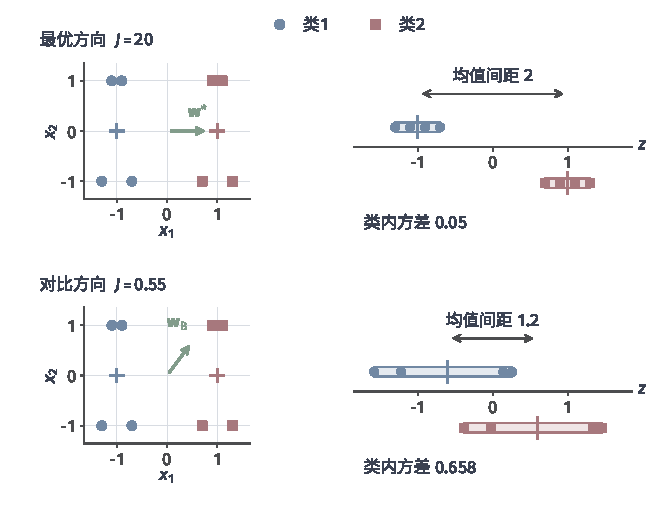
\includegraphics[width=112.000mm]{figures/04-classic-models/00-shared/matplotlib/classification-lda-target/figure.pdf}
  \caption{Fisher投影同时比较均值间距与类内散布。每类4个教学点，坐标无量纲；两行复用同一点集和相同投影数轴尺度。左侧绿色箭头为单位投影方向，十字为类均值；右侧短竖线为投影均值，浅色条为各类的样本投影范围，双向箭头标出均值间距。标注方差由$n^{-1}\bm w^{\top}\bm S_{\mathrm W}\bm w$计算，$J$仍按散度比计算。}
  \label{fig:classification-lda-projection}
\end{figure}

由于$J$不受$\bm{w}$的非零倍数缩放影响，可以约束$\bm{w}^{\top}\bm{S}_{\mathrm{W}}\bm{w}=1$。对$\bm{w}^{\top}\bm{S}_{\mathrm{B}}\bm{w}-\lambda(\bm{w}^{\top}\bm{S}_{\mathrm{W}}\bm{w}-1)$求导，得到\term{广义特征值问题}（generalized eigenvalue problem）：
\begin{equation}
  \label{eq:classification-fisher-eigenproblem}
  \bm{S}_{\mathrm{B}}\bm{w}
    =\lambda\bm{S}_{\mathrm{W}}\bm{w}.
\end{equation}
驻点还需比较大小。令$\bm{v}=\bm{S}_{\mathrm{W}}^{1/2}\bm{w}$，则
\[
  J(\bm{w})=\frac{\bm{v}^{\top}\bm{A}\bm{v}}{\bm{v}^{\top}\bm{v}},
  \qquad
  \bm{A}=\bm{S}_{\mathrm{W}}^{-1/2}
    \bm{S}_{\mathrm{B}}\bm{S}_{\mathrm{W}}^{-1/2}.
\]
把$\bm{v}$展开到对称半正定矩阵$\bm{A}$的正交特征向量上，上式就是各特征值的加权平均，权重非负且总和为$1$。最大值因而是最大特征值；取对应特征向量，再乘$\bm{S}_{\mathrm{W}}^{-1/2}$，便得到最优Fisher方向。若最大特征值有重数，最优方向未必唯一。

二分类时，令$\bm{h}=\hat{\bm{\mu}}_1-\hat{\bm{\mu}}_2\ne\bm{0}$，由总均值的定义可得
\[
  \bm{S}_{\mathrm{B}}=\frac{n_1n_2}{n}\bm{h}\bm{h}^{\top},
  \qquad
  \bm{w}_{\mathrm{F}}\propto\bm{S}_{\mathrm{W}}^{-1}\bm{h}.
\]
生成式LDA的法向量则为$\bm{w}_{\mathrm{G}}=\hat{\bm{\Sigma}}^{-1}\bm{h}=n\bm{S}_{\mathrm{W}}^{-1}\bm{h}$，两者方向相同。但完整的生成式分类规则还比较
\begin{equation}
  \label{eq:classification-lda-binary-threshold}
  \hat\delta_1(\bm{x})-\hat\delta_2(\bm{x})
    =\bm{w}_{\mathrm{G}}^{\top}
      \left(\bm{x}-\frac{\hat{\bm{\mu}}_1+\hat{\bm{\mu}}_2}{2}\right)
      +\log\frac{\hat\pi_1}{\hat\pi_2}
\end{equation}
的正负。Fisher准则本身只给方向，不给类先验、后验概率或这一阈值。两类均值相同时，均值散度准则没有正特征值方向，而生成模型仍可按先验选择类别。因此Fisher投影可用于非高斯数据，而贝叶斯最优性的证明还需要正确指定的高斯生成模型。

\subsubsection{理论分析}
\label{sec:classification-lda-analysis}

\paragraph{表达能力}
若真实类条件分布满足式\eqref{eq:classification-lda-distribution}，其后验概率就属于LDA的候选概率函数集，相应的贝叶斯决策也属于候选分类规则，无须用近似模型代替。共享协方差允许相关特征和不同类中心，但规定各类只有一个高斯峰，且峰周围的形状相同。即使不把得分解释为高斯后验，两个仿射得分的比较也只能产生一个半空间，不能表达任意形状的类别区域。

前面的同中心例子可以具体写成两类等先验、均值均为零，协方差分别为$\sigma_1^2\bm I_d$与$\sigma_2^2\bm I_d$，其中$0<\sigma_1<\sigma_2$。比较真实高斯密度得到：类1的贝叶斯区域是
\[
  \|\bm x\|_2^2<r_0^2,
  \qquad
  r_0^2=\frac{2d\log(\sigma_2/\sigma_1)}
                   {\sigma_1^{-2}-\sigma_2^{-2}}.
\]
小方差类在中心附近占优，大方差类在外侧占优。LDA的每个二类候选规则都以半空间作为类别区域，因而无法重现这个有界球。QDA保留半径平方项，候选空间能够表达这里的目标区域；两者的区别落在得分中是否允许这项二次关系。

\paragraph{收敛性}
固定训练集、各类别非空且类内散度正定时，生成式LDA的闭式参数达到该高斯模型的经验似然全局最大值，不需要迭代搜索。累积散度约需$O(nd^2)$运算，分解协方差约需$O(d^3)$运算；奇异情形没有这一正定域内的有限最优解。Fisher投影则通过广义特征值求解达到其比值准则的全局最大值，数值精度与矩阵条件数有关。

\paragraph{泛化性}
闭式估计只解决当前训练集上的拟合。下面先证明参数估计的\term{一致性}（consistency），再说明这些参数构成的分类器能否接近贝叶斯风险。给定训练集$D_n$后，$R(f\mid D_n)$只对独立新样本取平均。

\begin{lemma}[LDA参数估计的一致性]
  \label{thm:classification-lda-consistency}
  设$d$和$C$固定，训练样本独立同分布，真实分布满足式~\eqref{eq:classification-lda-distribution}，且所有$\pi_c^\ast>0$、$\bm{\Sigma}^\ast\succ0$。当$n\to\infty$时，
  \[
    \hat\pi_c\xrightarrow{\mathbb{P}}\pi_c^\ast,\qquad
    \hat{\bm{\mu}}_c\xrightarrow{\mathbb{P}}\bm{\mu}_c^\ast,\qquad
    \hat{\bm{\Sigma}}\xrightarrow{\mathbb{P}}\bm{\Sigma}^\ast .
  \]
  所有类别非空且$\hat{\bm{\Sigma}}$正定的概率趋于$1$。
\end{lemma}

\begin{proof}
  为处理随机的$n_c$，把类均值写成两个全样本平均之比：
  \[
    \hat{\bm{\mu}}_c
      =\frac{n^{-1}\sum_{i=1}^{n}\bm{x}_i\mathbb{1}\{y_i=c\}}
        {n^{-1}\sum_{i=1}^{n}\mathbb{1}\{y_i=c\}} .
  \]
  大数定律使分母收敛到$\pi_c^\ast>0$，分子收敛到$\pi_c^\ast\bm{\mu}_c^\ast$，因而先验和均值都一致。尚未观察到某一类时可以任意约定其均值；该事件的概率趋于零，不影响结论。

  共享协方差估计可展开为
  \[
    \hat{\bm{\Sigma}}
      =\frac1n\sum_{i=1}^{n}\bm{x}_i\bm{x}_i^{\top}
        -\sum_{c=1}^{C}\hat\pi_c
          \hat{\bm{\mu}}_c\hat{\bm{\mu}}_c^{\top}.
  \]
  高斯分布有有限二阶矩，故第一项收敛到
  \[
    \mathbb{E}[\bm{x}\bm{x}^{\top}]
      =\bm{\Sigma}^\ast+
        \sum_{c=1}^{C}\pi_c^\ast
          \bm{\mu}_c^\ast(\bm{\mu}_c^\ast)^{\top}.
  \]
  第二项消去类中心对二阶矩的贡献，余下$\bm{\Sigma}^\ast$。固定维数下，矩阵逐元素收敛也给出算子范数收敛；由$\bm{\Sigma}^\ast$的最小特征值严格为正，估计矩阵以趋于$1$的概率可逆。上述步骤实际上可由强大数定律加强为几乎必然收敛。
\end{proof}

矩阵求逆和$\log\pi_c$在这些条件下连续，所以在参数几乎必然收敛的事件上，对每个固定输入$\bm{x}$，有$\hat\delta_c(\bm{x})\to\delta_c^\ast(\bm{x})$。但$\argmax$在平局处不连续：在真实最大得分唯一的输入处，估计类别最终等于该输入的唯一贝叶斯类别；平局处则未必如此。若最优类别平局的输入集合概率为零，就能进一步推出随机输入上的预测标签收敛。不同贝叶斯分类器在平局处可以选择不同标签，却有相同风险。

参数收敛怎样传到预测错误率，可以直接通过类别后验比较，因而不需要排除后验平局。
\begin{theorem}[LDA在高斯同协方差条件下的期望分类风险界]
  \label{thm:classification-lda-risk}
  在引理\ref{thm:classification-lda-consistency}的条件下，用闭式估计的先验、均值和共享协方差构造$\hat p_c$，返回$\hat f_{\mathrm{LDA}}=\argmax_c\hat p_c$，平局按固定类别次序处理。不能拟合的训练集上暂用任意固定分类器。记真实后验为$p_c^\ast$，则在估计模型有定义时，
  \[
    0\leq R(\hat f_{\mathrm{LDA}}\mid D_n)-R^\ast
      \leq2\mathbb E_{\bm X}
        \max_c|\hat p_c(\bm X)-p_c^\ast(\bm X)|.
  \]
  随$n\to\infty$，左侧几乎必然趋于零，而且
  $\mathbb E_{D_n}R(\hat f_{\mathrm{LDA}}\mid D_n)\to R^\ast$。
\end{theorem}
\begin{proof}
记$f^\ast$为任意贝叶斯规则。由于$\hat f_{\mathrm{LDA}}$最大化$\hat p_c$，逐点有
\begin{equation}
  \label{eq:classification-lda-excess-risk}
  \begin{aligned}
    0&\leq p_{f^\ast(\bm{x})}^\ast(\bm{x})
      -p_{\hat f_{\mathrm{LDA}}(\bm{x})}^\ast(\bm{x})\\
      &\leq 2\max_{1\leq c\leq C}
          |\hat p_c(\bm{x})-p_c^\ast(\bm{x})| .
  \end{aligned}
\end{equation}
这个上界来自在两项之间分别加减相应的估计后验，并利用$\hat p_{\hat f_{\mathrm{LDA}}}\geq\hat p_{f^\ast}$。对独立测试输入积分，左侧成为超额风险，得到定理中的不等式。在参数几乎必然收敛的事件上，后验估计对每个输入收敛，右端的被积函数趋于零且不超过$2$；支配收敛定理给出条件风险的极限。再用风险位于$[0,1]$，对训练集取期望即可得到最后一个结论。由参数一致性引理，不能拟合的事件几乎必然最终不再出现。
\end{proof}

这条推理从训练统计量出发，经后验误差控制到独立新样本风险，依赖正确指定的高斯模型与固定维数。它给出风险极限，未给出有限样本速率；维数随样本量增长时也需另外分析。Fisher准则只评价投影的散度比例，没有这些分布条件时，不能由它推出上述风险结论。

\subsubsection{优化表达能力}

\paragraph{允许各类具有不同协方差}
\label{sec:classification-lda-covariance-extensions}
如果不同类别的类内变化方向和尺度明显不同，共享协方差就会限制LDA的表达能力。第\ref{sec:classification-lda-model}节已经定义的二次判别分析（QDA）保留类条件高斯假设，却为每个类别估计独立的协方差矩阵$\hat{\bm{\Sigma}}_c$。先假设各类协方差估计均正定，删去各类共同的常数项后，其判别得分为
\begin{equation}
  \begin{aligned}
    \delta_c(\bm{x})
      ={}&\log\hat{\pi}_c-\frac12\log\det\hat{\bm{\Sigma}}_c\\
        &-\frac12(\bm{x}-\hat{\bm{\mu}}_c)^\top
          \hat{\bm{\Sigma}}_c^{-1}(\bm{x}-\hat{\bm{\mu}}_c).
  \end{aligned}
  \label{eq:classification-qda-score}
\end{equation}
任意两类得分之差含有关于$\bm{x}$的二次项，所以边界一般是二次曲面。当协方差相同时，二次项相消，又得到 LDA。增加自由度也增加了估计负担：共享协方差模型需要$O(d^2+Cd)$个参数，QDA 则需要$O(Cd^2)$个参数；每一类只有少量样本时，独立协方差容易不稳定甚至奇异。第\ref{sec:classification-gda}节将从生成分布的角度统一这两种模型。

\paragraph{支持非线性关系}
\label{sec:classification-lda-kernel-extension}
QDA通过类协方差的差异产生二次边界；Fisher判别则可以从输入表示入手，改变只作线性投影的限制。例如，内外两圈样本在原坐标中的均值都可能接近原点，原坐标上的均值差便提供不了有用方向；增加距离平方等非线性特征后，两类在新坐标中可以具有不同均值。Mika等提出的\term{核 Fisher 判别}（kernel Fisher discriminant, KFD）在特征空间中重新计算类均值与散度，再最大化投影后的类间与类内散度比\scite{mika1999kernel}。
将投影方向写成$\bm{w}=\sum_{i=1}^n a_i\phi(\bm{x}_i)$，两种投影散度就都能写成系数$\bm{a}$与核矩阵构成的二次型，目标仍是它们的比值；类内散度的奇异性则用正则化处理。它与核 SVM 的区别仍在训练准则：KFD 关注整体类统计量，SVM 关注间隔及其违反程度。KFD 的基本解通常没有支持向量式的稀疏性，预测可能需要访问全部训练样本；若要从投影得分得到后验概率，还需额外建立得分分布或校准模型。
例如，内外两圈分别具有固定半径$1$与$2$时，径向特征$\phi(\bm x)=\|\bm x\|_2^2$把两类送到$1$与$4$。在二者之间设置阈值就能精确分开，带正则化的类内散度也不妨碍这个得分表示。若所选核仍只提供原坐标的线性组合，同中心两圈的均值差仍为零，Fisher准则便没有得到所需的径向信息。所选核是否保留径向信息，决定了这里的目标能否表达。

\subsubsection{优化泛化能力}

QDA放开了各类的形状，但少数类可能没有足够样本估计完整协方差。例如，一个类别只有10个样本，中心化后的样本协方差秩至多为9；若输入有20维，这个估计便无法求逆。完全改用LDA又会舍弃类间真实的尺度或方向差异。可以在两者之间折中，让各类借用一部分合并统计量。\term{正则化判别分析}（regularized discriminant analysis, RDA）通过收缩协方差控制这种取舍。Friedman的原始方法包含两个调节方向：将类内协方差向合并协方差收缩，再向球形协方差收缩\scite{friedman1989rda}。
记$n_c$为第$c$类样本数，$\hat{\bm{\Sigma}}$为以$n$为分母的合并协方差。一种与原始构造相符的写法是
\begin{equation}
  \begin{aligned}
    \bm{A}_c(a)
      &=\frac{(1-a)n_c\hat{\bm{\Sigma}}_c+an\hat{\bm{\Sigma}}}
              {(1-a)n_c+an},\\
    \tilde{\bm{\Sigma}}_c(a,b)
      &=(1-b)\bm{A}_c(a)
        +b\,\frac{\operatorname{tr}\bm{A}_c(a)}{d}\bm{I},
        \qquad a,b\in[0,1].
  \end{aligned}
  \label{eq:classification-rda}
\end{equation}
当$b=0$时，$a=0$与$a=1$分别对应 QDA 与 LDA 的协方差估计；增大$b$会减弱各方向方差差异，并在平均方差为正时帮助获得可逆估计。两个参数应在训练集内部通过验证选择。当合并协方差和各类协方差均奇异时，可逆性还需要平均方差为正的球形收缩项或其他正则化。

收缩也改变哪些类别差异能够进入得分。$a=1,b=0$时各类共享协方差，二次项相消；$b=1$时每类协方差都为单位矩阵的一个倍数，得分可以利用半径平方，却不能独立利用各方向的方差与特征相关性。只有保留完整的类特有协方差，才能表达前面QDA中的一般二次差异。RDA是在这些限制与估计波动之间选择，不是一个可以越过QDA分布族的新模型。

收缩强度越大，类形状越受限制；强度越小，越依赖每类样本估计完整协方差。应在训练数据内部选择强度，再检查独立数据上的分类误差与估计稳定性。

\subsubsection{小结}
\label{sec:classification-lda-summary}

LDA把类中心、类内波动与类别比例合成一个得分。共享协方差使两类比较中的二次项抵消，留下线性边界；高斯生成模型还给出后验与阈值。Fisher的投影准则则把均值分离和类内散布放在同一个比值中，适合解释各特征怎样参与判别，但只选方向，不能独自给出后验概率。

类形状不同时，QDA保留各类协方差，代价是每类都要有足够数据支持矩阵估计。小样本、高维条件下，Friedman的RDA让各类借用合并统计量，再按需要向球形协方差收缩，减轻独立估计的波动。收缩越强，能够保留的方向与尺度差异越少；收缩参数的选择也增加了验证工作。

另一类困难来自原坐标没有显示类别差异。内外两圈的均值可以相同，单纯调整协方差估计无法为线性Fisher投影补上径向关系。Mika等的核Fisher判别把类统计量移到特征空间，让非线性关系进入同一个散度准则。代价是核矩阵、散度正则化与通常较稠密的预测表示；核所保留的信息仍决定哪些目标能够表达。若任务需要多个判别方向，相关降维构造见第\ref{chap:dimensionality-reduction}章。

\subsection{感知机}
\label{sec:classification-perceptron}

LDA先估计每类分布，再由这些分布决定边界。若任务只要求给出类别，我们也可以直接用预测错误调整边界。例如，两类点虽然可以被一条直线分开，却沿不同方向伸展，不适合共享协方差的描述。寻找分隔线仍是有意义的任务，并不需要先把每类的分布拟合好。

\term{感知机}（perceptron）从一组初始权重出发，逐个检查训练样本；遇到分类条件被违反的样本，就沿提高其正确类别得分的方向修正权重。这样，标签直接告诉算法边界需要怎样移动。算法可在任意训练集上运行；若训练集具有正间隔可分性，才有后面证明的有限更新保证。Rosenblatt在1958年的论文中研究了这一学习机制，本节介绍其中广泛使用的线性阈值模型与误差修正规则\scite{rosenblatt1958}。

康奈尔航空实验室还用Mark I Perceptron将这一研究路线实现为电子装置。历史系统包含感觉、关联和响应等组织；本节抽取的是后来常用的单个线性分类器及其更新规则\scite{smithsonianMarkI}。

\subsubsection{模型结构}
\label{sec:classification-perceptron-model}

本小节先使用二分类标签$y_i\in\{-1,+1\}$。为了使偏置在更新规则和收敛证明中始终处于同一坐标系，引入\term{增广向量}（augmented vector），即在输入末尾补一个恒为$1$的分量，并把偏置并入参数：
\begin{equation}
  \label{eq:classification-perceptron-augmented}
  \tilde{\bm{x}}=
    \begin{pmatrix}\bm{x}\\1\end{pmatrix},\qquad
  \tilde{\bm{w}}=
    \begin{pmatrix}\bm{w}\\b\end{pmatrix}
    \in\mathbb{R}^{d+1}.
\end{equation}
其中$\bm{w}\in\mathbb{R}^{d}$，$b\in\mathbb{R}$。分类规则为
\begin{equation}
  \label{eq:classification-perceptron-prediction}
  f(\bm{x})=\operatorname{sign}
    (\tilde{\bm{w}}^{\top}\tilde{\bm{x}})
    =\operatorname{sign}(\bm{w}^{\top}\bm{x}+b).
\end{equation}
约定$\operatorname{sign}(s)=+1$当$s\geq0$，否则为$-1$。非退化边界$\bm{w}^{\top}\bm{x}+b=0$是在$d$维输入空间中的$(d-1)$维超平面。它与二分类LDA具有相同的边界形式；这里的参数来自错误反馈，输出是类别得分与标签，概率需要另建模型。

在这一表示下，正间隔可分是指存在单位向量$\bm{u}^\ast\in\mathbb{R}^{d+1}$和$\gamma>0$，使
\begin{equation}
  \label{eq:classification-perceptron-margin}
  \begin{aligned}
    y_i\langle\bm{u}^\ast,\tilde{\bm{x}}_i\rangle
      &\geq\gamma,\qquad i=1,\ldots,n,\\
    \|\bm{u}^\ast\|_2&=1,\qquad
    \|\tilde{\bm{x}}_i\|_2\leq R .
  \end{aligned}
\end{equation}
这里$R$约束的是增广输入，因此$R\geq\max_i\sqrt{\|\bm{x}_i\|_2^2+1}$。$\gamma$也是增广空间中的间隔；若$\bm{u}^\ast=(\bm{v}^{\top},a)^{\top}/\sqrt{\|\bm{v}\|_2^2+a^2}$，其分母包含偏置$a$，不同于原输入空间中以$\|\bm{v}\|_2$归一化的几何距离。有限训练集只要能被仿射超平面严格分开，就存在这样的正$\gamma$。

线性表示的边界也很具体。例如异或任务把$(0,0)$、$(1,1)$标为负类，把$(1,0)$、$(0,1)$标为正类。按上述平局规则，前两点要求$b<0$和$w_1+w_2+b<0$，后两点要求$w_1+b\geq0$和$w_2+b\geq0$。前两式相加与后两式相加，对同一个$w_1+w_2+2b$给出矛盾要求。Minsky与Papert在1969年的《Perceptrons》中系统研究了此类表示能力限制；改变输入特征或加入非线性隐藏层可以越过单个线性边界的限制，但那已经改变了模型族\scite{minsky1969}。

\subsubsection{参数学习}
\label{sec:classification-perceptron-learning}

从$\tilde{\bm{w}}^{(0)}=\bm{0}$出发，若当前样本满足$y_i\langle\tilde{\bm{w}}^{(t)},\tilde{\bm{x}}_i\rangle\leq0$，便进行一次更新：
\begin{equation}
  \label{eq:classification-perceptron-update}
  \tilde{\bm{w}}^{(t+1)}
    =\tilde{\bm{w}}^{(t)}+\eta y_i\tilde{\bm{x}}_i,
    \qquad \eta>0 .
\end{equation}
这里$t$只数实际更新，学习率$\eta$保持不变。拆开最后一个分量，就是$\bm{w}\leftarrow\bm{w}+\eta y_i\bm{x}_i$和$b\leftarrow b+\eta y_i$。同一个样本的有符号得分增加$\eta\|\tilde{\bm{x}}_i\|_2^2$，所以更新确实朝修正当前判断的方向移动；但它可能同时破坏其他样本的正确分类，因而需要反复遍历。零得分也触发更新，即使按平局规则恰好预测为正确的正类，仍要求它离开边界。

图~\ref{fig:classification-perceptron-update}把这一步写成具体数值。取当前参数$\bm w=(1,0)^{\top}$、$b=-1$，正类点$\bm x_i=(0.5,1)^{\top}$的得分为$-0.5$，触发更新。学习率为$0.5$时，权重变为$(1.25,0.5)^{\top}$，偏置变为$-0.5$，当前点的得分增加到$0.625$。图中边界因此同时改变位置和方向；判断是否继续更新，仍要逐个检查后续样本。

\begin{figure}[htbp]
  \centering
  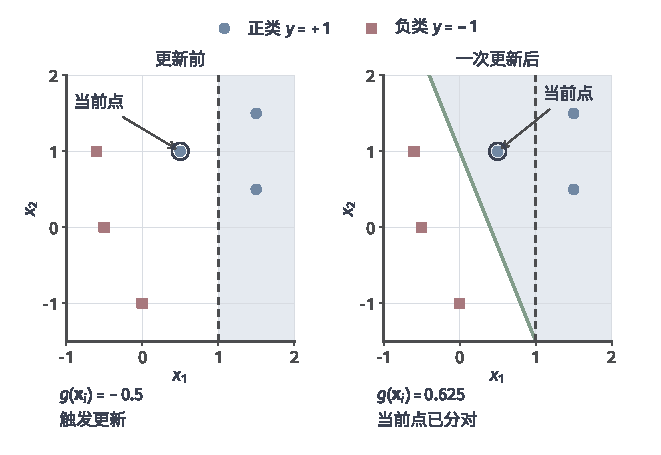
\includegraphics[width=112.000mm]{figures/04-classic-models/00-shared/matplotlib/classification-perceptron-update/figure.pdf}
  \caption{错分正类点触发的一次感知机更新。六个点为教学构造，坐标无量纲，两面板共用坐标范围；蓝圆、红方分别为正负类，黑色圆环标出当前点。浅蓝区域为正类预测区域，虚线为旧边界$x_1=1$，绿色实线为新边界$1.25x_1+0.5x_2=0.5$。偏置随权重一起更新，当前点由负得分变为正得分。}
  \label{fig:classification-perceptron-update}
\end{figure}

\begin{algorithm}[带遍历上限的感知机训练]
  \label{alg:classification-perceptron}
  \begin{algorithmic}[1]
    \Require $D_n$，固定学习率$\eta>0$，最大遍历轮数$E\geq1$
    \Ensure 参数$\tilde{\bm{w}}$与是否已验证收敛的状态
    \State $\tilde{\bm{w}}\gets\bm{0}$
    \For{$e=1,\ldots,E$}
      \State $m\gets0$
      \For{$i=1,\ldots,n$}
        \State $\tilde{\bm{x}}_i\gets(\bm{x}_i^{\top},1)^{\top}$
        \If{$y_i\langle\tilde{\bm{w}},\tilde{\bm{x}}_i\rangle\leq0$}
          \State $\tilde{\bm{w}}\gets\tilde{\bm{w}}+\eta y_i\tilde{\bm{x}}_i$
          \State $m\gets m+1$
        \EndIf
      \EndFor
      \If{$m=0$}
        \State \Return $(\tilde{\bm{w}},\text{已收敛})$
      \EndIf
    \EndFor
    \State \Return $(\tilde{\bm{w}},\text{达到轮数上限})$
  \end{algorithmic}
\end{algorithm}

一整轮没有更新时，所有样本都是在同一个参数下得到严格正的有符号得分，才构成收敛证据。达到轮数上限时返回的是预算内的当前解，可分性仍未由这一停止状态判定。稠密实现每轮需要$O(nd)$运算，除训练集外只需$O(d)$参数空间；样本访问顺序可以改变输出的分隔面。

从优化角度看，定义\term{感知机损失}（perceptron loss）
\begin{equation}
  \label{eq:classification-perceptron-loss}
  \ell_{\mathrm{P}}(\tilde{\bm{w}};\bm{x}_i,y_i)
    =\max\{0,-y_i\langle\tilde{\bm{w}},\tilde{\bm{x}}_i\rangle\}.
\end{equation}
为了把这项损失用于更新，先看它的两段：当带符号得分为负时，对参数求导得到$-y_i\tilde{\bm{x}}_i$；得分为正时，损失恒为零，梯度也是$\bm 0$。两段在零得分处相接，却给出不同斜率，普通梯度在这里没有定义。由于损失仍是凸的，可以使用次梯度；在交点处选择$-y_i\tilde{\bm{x}}_i$，仍满足支撑损失的仿射下界条件，也就得到式~\eqref{eq:classification-perceptron-update}。这一求解依据见\BookSectionRef{sec:opt-subgradient-methods}{第一卷“数学准备”的“基于次梯度的求解”节}。

上述更新逐样本执行；随机抽取样本时才相应成为随机次梯度下降。这里使用的是零间隔损失，不是标准的\term{合页损失}（hinge loss）$\max\{0,1-y_i\langle\tilde{\bm{w}},\tilde{\bm{x}}_i\rangle\}$。前者在零参数处就对所有样本取零，因此“感知机损失为零”本身不能证明分类正确；算法在零得分处仍更新的约定不可省略。

\subsubsection{理论分析}
\label{sec:classification-perceptron-analysis}

\paragraph{表达能力}
单层感知机的候选规则为$\operatorname{sign}(\bm w^\top\bm x+b)$。目标本来就是一个半空间时，这个候选类可以精确表示它；目标依赖特征交互时，则可能无法同时满足全部类别条件。

例如，取$(1,1)$、$(-1,-1)$、$(1,-1)$、$(-1,1)$四点作为输入域，同号坐标的目标标签为$-1$，异号坐标为$+1$。正、负两对点的中点都在原点。若一个仿射得分把四点全分对，正类得分的平均必须非负，负类得分的平均必须为负；两者却都等于$b$，产生矛盾。因此候选类中的每个函数至少在一个点上偏离目标。增加特征$x_1x_2$后，得分$-x_1x_2$恰好满足四点的目标标签，这才改变了候选空间的表示限制。

\paragraph{收敛性}
每次修正可能破坏已有判断，为什么这些修正不会无穷持续？关键是存在一个始终把所有样本分对的参考方向：更新朝该方向取得线性累积的进展，而参数范数的平方只能线性增长。Novikoff在1962年报告的证明清楚展示了这两个增长速度之间的矛盾\scite{novikoff1962}。

\begin{theorem}[感知机在有界可分样本下的最大更新次数]
  \label{thm:classification-perceptron-mistakes}
  若$D_n$满足式~\eqref{eq:classification-perceptron-margin}，从零参数出发，以固定$\eta>0$按式~\eqref{eq:classification-perceptron-update}更新，则对任意样本访问顺序，错误更新次数$M$满足
  \[
    M\leq\left(\frac R\gamma\right)^2 .
  \]
  这里错误更新包括零得分时的更新。若持续完整遍历训练集，且不因预算提前退出，算法在有限轮后得到所有训练样本上有符号得分均严格为正的参数。
\end{theorem}

\begin{proof}
  设第$t+1$次更新使用样本$i_t$。沿单位参考方向$\bm{u}^\ast$考察更新，得到
  \begin{align*}
    \langle\tilde{\bm{w}}^{(t+1)},\bm{u}^\ast\rangle
      &=\langle\tilde{\bm{w}}^{(t)},\bm{u}^\ast\rangle
        +\eta y_{i_t}\langle\tilde{\bm{x}}_{i_t},\bm{u}^\ast\rangle\\
      &\geq\langle\tilde{\bm{w}}^{(t)},\bm{u}^\ast\rangle+\eta\gamma .
  \end{align*}
  从零参数累加$M$次，便有
  \[
    \langle\tilde{\bm{w}}^{(M)},\bm{u}^\ast\rangle
      \geq M\eta\gamma .
  \]
  另一方面，展开更新后的平方范数：
  \begin{align*}
    \|\tilde{\bm{w}}^{(t+1)}\|_2^2
      &=\|\tilde{\bm{w}}^{(t)}\|_2^2
        +2\eta y_{i_t}
          \langle\tilde{\bm{w}}^{(t)},\tilde{\bm{x}}_{i_t}\rangle\\
      &\quad+\eta^2\|\tilde{\bm{x}}_{i_t}\|_2^2\\
      &\leq\|\tilde{\bm{w}}^{(t)}\|_2^2+\eta^2R^2 .
  \end{align*}
  不等式使用了更新条件：交叉项非正；并使用同一增广空间中的长度界$R$。再次累加，得到$\|\tilde{\bm{w}}^{(M)}\|_2^2\leq M\eta^2R^2$。由Cauchy--Schwarz不等式和$\|\bm{u}^\ast\|_2=1$，
  \[
    M\eta\gamma
      \leq\langle\tilde{\bm{w}}^{(M)},\bm{u}^\ast\rangle
      \leq\|\tilde{\bm{w}}^{(M)}\|_2
      \leq\eta R\sqrt{M}.
  \]
  $M=0$时结论直接成立；$M>0$时除以$\eta\sqrt M$再平方，得到所述界。因此更新不可能无限发生。持续完整遍历会在最后一次更新之后再检查所有样本；若仍有非正得分就还会更新，产生矛盾，故最终必有一整轮没有更新。
\end{proof}

这个界不显式含$n$，也不依赖访问顺序，但$R$和$\gamma$随数据而定；增加样本可能缩小可分间隔。它只约束更新次数，不包括寻找错误时检查正确样本的开销。对于算法~\ref{alg:classification-perceptron}的逐轮扫描，若不提前截断，至多需要$M+1$轮，包括最终的无更新确认轮。

若数据不可分，有限更新保证失效，持续遍历可能反复更新，此时可以限制训练预算并保留历史较好解，或采用允许间隔违约的在线方法。这些处理改变了停止或选解方式，仍须分别分析。

\paragraph{泛化性}
测试风险需要训练更新之外的统计条件。前述错误次数证明只考察给定样本的几何结构；若要判断未来预测，需要规定抽样分布与训练后返回哪个分类器。Cesa-Bianchi、Conconi与Gentile在2004年研究了这种联系：由独立同分布样本上的在线表现控制历史预测规则的风险，并讨论相应的输出选择方法\scite{cesabianchi2004generalization}。

下面给出一个期望风险的简单结论，说明额外条件怎样进入证明。按独立同分布的到达顺序，仅遍历$D_n$一次，从零参数出发使用固定学习率$\eta>0$和原更新规则。用$f_i$表示看到第$i$个样本之前的分类器；它只依赖$D_{i-1}$，其中$D_0$为空。这里$i$计数已访问的样本位置，与只计实际更新的$t$不同。训练后独立地从$\{1,\ldots,n\}$均匀抽取$I$，返回$f_I$，使输出规则与下述期望风险证明一致。

\begin{theorem}[感知机随机历史输出在可分分布下的期望风险界]
  \label{thm:classification-perceptron-risk}
  设训练样本独立同分布，测试样本独立来自同一分布。假设存在固定的单位向量$\bm{u}^\ast$及常数$R<\infty$、$\gamma>0$，使
  \[
    \|\tilde{\bm{x}}\|_2\leq R,\qquad
    y\langle\bm{u}^\ast,\tilde{\bm{x}}\rangle\geq\gamma
    \quad\text{几乎必然}.
  \]
  对上述单遍历训练和随机输出规则，有
  \begin{equation}
    \label{eq:classification-perceptron-risk}
    \mathbb{E}_{D_n,I}\!\left[R(f_I\mid D_n,I)\right]
      \leq\frac{R^2}{n\gamma^2}.
  \end{equation}
\end{theorem}

\begin{proof}
  令$e_i=\mathbb{1}\{f_i(\bm{x}_i)\ne y_i\}$。由于$f_i$尚未使用第$i$个样本，独立性给出
  \[
    \mathbb{E}[e_i\mid D_{i-1}]
      =R(f_i\mid D_{i-1}).
  \]
  对两边取期望，再对均匀的$I$平均，就有
  \[
    \mathbb{E}_{D_n,I}[R(f_I\mid D_n,I)]
      =\frac1n\sum_{i=1}^{n}\mathbb{E}[e_i].
  \]
  每次预测错误都会触发更新，零得分且预测正确时也可能更新，故$\sum_i e_i\leq M$。分布层面的共同间隔和长度界使定理~\ref{thm:classification-perceptron-mistakes}几乎必然适用于每个训练序列，于是$M\leq R^2/\gamma^2$，代入即得结论。
\end{proof}

这里的$R$和$\gamma$约束整个数据分布。式~\eqref{eq:classification-perceptron-risk}对训练抽样及随机历史状态取平均；当上界小于$1$时，它提供非平凡的期望风险控制。最终参数或多轮训练使用不同的输出与依赖关系，需各自分析：尤其在多轮中，当前样本已经参与既有参数的形成。不同的历史选解规则需要分别检查其训练依赖。

\subsubsection{优化表达能力}

若问题在于原空间不能线性分开，可把输入换成特征映射$\bm{\phi}(\bm{x})$。核函数$K(\bm{x},\bm{z})=\langle\bm{\phi}(\bm{x}),\bm{\phi}(\bm{z})\rangle$直接计算映射后的内积，省去显式构造高维坐标，得到\term{核感知机}（kernel perceptron）。为与前文偏置一致，使用增广映射$(\bm{\phi}(\bm{x}),1)$及其核$\tilde K(\bm{x},\bm{z})=K(\bm{x},\bm{z})+1$。零初始化、单位学习率下，参数在特征空间中是更新样本的线性组合，预测可写为
\begin{equation}
  \label{eq:classification-kernel-perceptron}
  f(\bm{x})=\operatorname{sign}
    \left(\sum_{i=1}^{n}\alpha_i y_i
      [K(\bm{x}_i,\bm{x})+1]\right).
\end{equation}
这里$\alpha_i$是样本$i$的更新次数；遇到非正有符号得分时令$\alpha_i\leftarrow\alpha_i+1$。必须选用正定核，即它在任意有限输入集上生成半正定Gram矩阵，才能作上述内积解释；有限更新还要求增广特征空间内存在正间隔，长度界相应变为$\sqrt{K(\bm{x}_i,\bm{x}_i)+1}$的上界。预测需要访问系数非零的样本，数量可能随训练增长。将内积推广到特征空间的思路可追溯至Aizerman、Braverman与Rozonoer在1964年的势函数研究\scite{aizerman1964}。

核与输入尺度共同决定映射后是否可分；预测成本则由需要保存的更新样本数决定。核化改变表示，不替代对标签噪声、停止规则和样本外误差的检查。

\subsubsection{优化泛化能力}

若希望减轻预测对最后一次参数更新的依赖，可以汇总训练过程中的多个状态。Freund与Schapire在1999年研究的\term{投票感知机}（voted perceptron）保存历次权重，并按各状态持续使用的次数加权投票；同一论文也比较了用历史得分平均代替投票的方式\scite{freund1999}。沿用本节的增广表示，设保存的状态为$\tilde{\bm w}_1,\ldots,\tilde{\bm w}_K$，$c_k>0$是第$k$个状态的计数，则投票预测为
\begin{equation}
  f_{\mathrm V}(\bm x)
  =\operatorname{sign}\!\left[
    \sum_{k=1}^{K}c_k\operatorname{sign}
       (\tilde{\bm w}_k^\top\tilde{\bm x})\right].
  \label{eq:classification-voted-perceptron}
\end{equation}
计数必须与更新同步。初始零参数的计数取零；本次检查未触发更新时，将当前状态的计数加一；触发更新时，保存新参数并把新状态的计数置为一，不再给被替换的旧状态加一。这里沿用非正有符号得分触发更新的约定，最后忽略计数为零的状态。计数取决于访问顺序与训练预算，并不是对新样本准确率的独立测量。保存与预测$K$个稠密状态均需考虑$O(Kd)$的代价。

\term{平均感知机}（averaged perceptron）改为先把这些增广参数平均：
\[
  \bar{\bm w}=\frac{\sum_{k=1}^{K}c_k\tilde{\bm w}_k}
                        {\sum_{k=1}^{K}c_k},
  \qquad
  f_{\mathrm A}(\bm x)=\operatorname{sign}
                    (\bar{\bm w}^\top\tilde{\bm x}).
\]
线性实现可在训练时累计参数和，最终只保存一组参数，额外存储与单次预测均为$O(d)$。投票先对每个得分取符号，再汇总标签；参数平均先汇总实值得分，再取符号，二者一般不同。前者的最终规则可以组合多个半空间判断，后者仍返回单个仿射得分；它们都改变训练结束后的输出方式，不能仅凭“汇总历史”判断哪种更适合任务。

\subsubsection{优化计算能力}

\paragraph{保存预算内的较优参数}
不可分数据可能使参数反复改变，预算结束时的权重未必是已经检查过的最好结果。\term{口袋算法}（Pocket algorithm）通过保存历史参数处理这个问题。常用版本额外保存$\tilde{\bm{w}}_{\mathrm{pocket}}$：每次检查候选参数时，计算全训练集零一错误数，仅在严格改进时替换记录；预算用尽后返回记录参数。它适用于噪声或矛盾标签数据，返回预算内已检查候选中的最小训练错误解；每次候选比较还需要评估全训练集。Gallant在1990年的论文中系统讨论了Pocket及相关学习方法\scite{gallant1990}。

Pocket只改变返回哪组历史参数，候选得分仍是原坐标中的仿射函数。它需要额外评估全部训练样本，也不能消除前面异或任务的表示限制。这里改善的是有限预算下的返回规则，并未使不可分数据上的原更新停止，也不保证找到所有仿射分类器中的最小训练错误解。

\paragraph{控制单步参数改动}
若希望每次更新不仅改正符号，还达到指定得分间隔，\term{被动攻击算法}（passive-aggressive algorithm, PA）把“尽量少改参数”和“满足当前样本的单位间隔”合成一个投影问题。用$\bm{v}$表示待求的新增广参数，
\begin{equation}
  \label{eq:classification-pa-projection}
  \begin{aligned}
    \min_{\bm{v}}\quad&
      \frac12\|\bm{v}-\tilde{\bm{w}}\|_2^2\\
    \text{满足}\quad&
      y_i\langle\bm{v},\tilde{\bm{x}}_i\rangle\geq1 .
  \end{aligned}
\end{equation}
令$\ell_i=\max\{0,1-y_i\langle\tilde{\bm{w}},\tilde{\bm{x}}_i\rangle\}$。约束已满足时参数不变；否则，拉格朗日驻点要求$\bm{v}=\tilde{\bm{w}}+\tau_i y_i\tilde{\bm{x}}_i$，将活跃约束代回即得
\[
  \tau_i=\frac{\ell_i}{\|\tilde{\bm{x}}_i\|_2^2},
  \qquad
  \tilde{\bm{w}}\leftarrow
    \tilde{\bm{w}}+\tau_i y_i\tilde{\bm{x}}_i .
\]
因此PA在间隔足够时“被动”，不足时按违约大小调整。增广方式也意味着这里把偏置变化纳入距离惩罚。噪声下硬性满足当前样本可能调整过大，PA-I可用$\tau_i=\min\{\lambda_{\mathrm{PA}},\ell_i/\|\tilde{\bm{x}}_i\|_2^2\}$限制步长，其中$\lambda_{\mathrm{PA}}>0$控制容忍程度。Crammer等人的2006年论文统一分析了这些在线大间隔方法；其保证针对在线更新的损失与间隔行为\scite{crammer2006}。
PA的单位间隔要求改变单步参数选择，候选得分仍是仿射函数。因此它与基本感知机、Pocket共享原坐标中的表示限制；间隔要求本身不能表达异或交互。

\subsubsection{支持多分类预测场景}

\label{sec:classification-perceptron-multiclass}

对$C$类问题，把标签改为$y_i\in\{1,\ldots,C\}$，每类维护一组增广参数$\tilde{\bm{w}}_c=(\bm{w}_c^{\top},b_c)^{\top}$，得分和预测为
\[
  s_c(\bm{x})=\langle\tilde{\bm{w}}_c,\tilde{\bm{x}}\rangle,
  \qquad
  \hat y=\argmax_{c\in\{1,\ldots,C\}}s_c(\bm{x}).
\]
平局仍按最小类别索引处理。这个构造把正确类别的得分与每个竞争类别作比较，也可用\term{Kesler构造}（Kesler construction）把这些比较写成一个扩展空间中的线性可分问题。

第$c$类获胜要求$s_c(\bm x)\geq s_j(\bm x)$对每个竞争类成立，平局处再按既定顺序处理。因此每类区域是若干半空间的交，仍是凸区域。它可以表示多类线性分区，却不能在原坐标中把某一类分成被其他类别隔开的多个区域；这种任务需要新的特征或不同的输出表示。

遇到$\hat y_i\ne y_i$时，只提高正确类别的参数并降低错误获胜类别的参数：
\begin{equation}
  \label{eq:classification-perceptron-multiclass-update}
  \begin{aligned}
    \tilde{\bm{w}}_{y_i}
      &\leftarrow\tilde{\bm{w}}_{y_i}+\eta\tilde{\bm{x}}_i,\\
    \tilde{\bm{w}}_{\hat y_i}
      &\leftarrow\tilde{\bm{w}}_{\hat y_i}-\eta\tilde{\bm{x}}_i .
  \end{aligned}
\end{equation}
其余类别不变，两个类别的偏置也随各自最后一个分量同时更新。若平局后预测错误，同样更新；若已选择正确类别，则该规则不更新。与二分类中所有零得分均更新的约定不同，这里直接按最终预测是否正确判断。

收敛条件也必须改为多类的得分差条件。把各类参数按行堆成$\tilde{\bm{W}}\in\mathbb{R}^{C\times(d+1)}$；假设存在$\|\bm{U}^\ast\|_{\mathrm{F}}=1$和$\gamma_{\mathrm{mc}}>0$，使对所有$i$和$c\ne y_i$都有
\[
  \langle\bm{U}_{y_i,:}^\ast-\bm{U}_{c,:}^\ast,
    \tilde{\bm{x}}_i\rangle\geq\gamma_{\mathrm{mc}} .
\]
这里$\|\cdot\|_{\mathrm{F}}$是所有矩阵元素平方和的平方根，行向量的内积按对应坐标计算。一次更新的方向矩阵仅两行非零，分别为$\tilde{\bm{x}}_i^{\top}$与$-\tilde{\bm{x}}_i^{\top}$，其平方范数至多为$2R^2$。它与$\bm{U}^\ast$的内积至少为$\gamma_{\mathrm{mc}}$；与当前参数的内积则为$s_{y_i}(\bm{x}_i)-s_{\hat y_i}(\bm{x}_i)\leq0$。因此零初始化时完全沿用二分类证明，得到
\[
  M\eta\gamma_{\mathrm{mc}}
    \leq\|\tilde{\bm{W}}^{(M)}\|_{\mathrm{F}}
    \leq\eta R\sqrt{2M},
  \qquad
  M\leq\frac{2R^2}{\gamma_{\mathrm{mc}}^2}.
\]
有限更新保证因而保留下来，但它要求所有正确类与竞争类之间都具有共同的正间隔，而不是只检查任意一对类别。

\subsubsection{支持结构化输出预测场景}

如果任务是给一句话中的每个词标注词性，输出就从一个类别变成了一整条标签序列。逐词独立判类无法在同一个得分中评价相邻标签的组合；我们希望同时比较不同候选序列，并在预测错误时调整整条序列用到的特征。\term{结构化感知机}（structured perceptron）把多分类的得分比较推广到结构之间，用联合特征$\bm{\phi}(\bm{x},y)$描述输入与候选结构，预测
\[
  \hat y_i=\argmax_{y\in Y(\bm{x}_i)}
    \langle\bm{\theta},\bm{\phi}(\bm{x}_i,y)\rangle ,
\]
其中$Y(\bm{x}_i)$是候选结构集合，$\bm{\theta}$是与联合特征同维的参数。解码错误时进行
\[
  \bm{\theta}\leftarrow\bm{\theta}
    +\eta\bigl[\bm{\phi}(\bm{x}_i,y_i)
      -\bm{\phi}(\bm{x}_i,\hat y_i)\bigr].
\]
联合特征决定哪些结构差异能够进入比较。若同一输入上的两个候选结构具有完全相同的$\bm\phi(\bm x,y)$，它们对所有参数都同分，候选得分无法区分两者，只能由固定的平局规则选择其中一个。词性标注中的相邻标签关系或更远处的依赖，因而需要由相应的特征记录；解码搜索再精确，也不能恢复特征没有保留的差异。

需要的类别或结构偏置也作为联合特征中的相应指示分量处理；对所有候选都相同的常数项会在得分差中消去。结构化输出增加了解码成本，近似解码还可能改变哪些样本触发更新，需要与特征设计一同评价。Collins在2002年将这种更新与参数平均用于序列标注，提供了词性标注和短语识别等实例，也为比较感知机与条件随机场等结构化模型提供了参照\scite{collins2002}。

\subsubsection{小结}
\label{sec:classification-perceptron-summary}

感知机用当前样本的标签直接修正边界，免去了先拟合类分布的步骤。一次更新提高当前样本的有符号得分，却可能改变其他样本的判断；因此样本顺序、停止预算和返回规则都属于实际学习过程。它提供简洁的增量训练方式，原坐标中的单个边界仍受仿射表示限制。

预算结束时怎样利用历史参数，是不可分或尚未收敛数据上的一个具体问题。Gallant讨论的Pocket保存已检查的较好状态，代价是重复评估训练集；Freund与Schapire的投票感知机让多个状态共同判类，代价是状态存储与多次预测。平均感知机把历史压缩成一组参数，减轻线性预测的负担，但它与标签投票采用不同的汇总规则。选择时需要比较同一访问顺序与预算下的分类误差和存储成本。

若缺的是非线性输入关系，核感知机把内积换到特征空间，预测则需要保留更新样本。PA处理的困难不同：当一步更新还不足以达到所需间隔时，Crammer等用最小参数改动满足当前约束，噪声下再限制过大的调整。它改变单步目标，原坐标中的表示仍然线性。

序列标注等结构化任务又需要改变输出比较。Collins的结构化感知机通过联合特征评价完整序列，解码成本随候选结构增加。输入表示、单步目标与输出结构解决不同困难，不能用增加遍历次数代替这些改变。

\subsection{支持向量机（SVM）}
\label{sec:classification-svm}

感知机回答了一个基本问题：如果训练样本能够被某个超平面分开，怎样通过错误驱动的更新找到一个分离器？但分开训练样本并不意味着分界的位置已经合适。同一批可分数据往往允许许多分离超平面，即使从零参数开始，感知机的结果仍会受样本顺序和更新规则影响。一个紧贴训练样本的边界虽然没有训练错误，却可能在输入受到很小扰动时改变预测。要在这些分离器之间作出选择，还需要说明什么样的边界更值得保留。

\term{支持向量机}（support vector machine，SVM）以训练样本到边界的距离选择分隔面：在正确分离样本的前提下，增大最近样本到边界的距离，称为最大间隔。给定特征表示与距离度量后，这个几何准则使边界具有可比较的尺度。不可分数据可以通过松弛约束处理，非线性关系则可以通过改变特征表示处理；两种扩展分别作用于误差容忍与候选函数。

核与松弛约束解决不同困难：Boser、Guyon与Vapnik在1992年把最大间隔训练与核表示结合，Cortes与Vapnik在1995年进一步系统发展了容许间隔违反的形式。前者改变非线性特征的使用方式，后者让噪声或类别重叠进入带惩罚的训练目标\scite{boser1992margin,cortes1995}。下面先从可分数据推导间隔目标与对偶，再用SMO说明参数怎样求出，最后分别改变输入表示、误差容忍和类别竞争。

\subsubsection{模型结构}
\label{sec:classification-svm-model}

沿用二分类标签约定，设训练集为$D_n=\{(\bm{x}_i,y_i)\}_{i=1}^n$，其中$\bm{x}_i\in\mathbb{R}^d$、$y_i\in\{-1,+1\}$，并假设两类均非空。令实值得分为$g(\bm{x})=\bm{w}^{\top}\bm{x}+b$，其中$\bm{w}\in\mathbb{R}^d$、$b\in\mathbb{R}$且$\bm{w}\ne\bm{0}$。决策超平面是$g(\bm{x})=0$，预测规则为$\hat y(\bm{x})=\operatorname{sign}(g(\bm{x}))$；若得分恰为零，约定预测为$+1$。

仅比较$y_i g(\bm{x}_i)$还不能比较不同超平面。把$(\bm{w},b)$同时乘以任意正数，分类结果不变，这个数值却会随之放大：同一条直线，把权重都乘以$100$，每个样本的得分也乘以$100$，直线却毫无变化。因此得分本身的“大小”带有任意性，不能直接当作距离或安全裕度。为区分参数尺度与真实距离，定义样本的\term{函数间隔}（functional margin）为$m_i=y_i g(\bm{x}_i)$，定义其\term{几何间隔}（geometric margin）为
\begin{equation}
  \gamma_i
  =\frac{y_i(\bm{w}^{\top}\bm{x}_i+b)}
         {\lVert\bm{w}\rVert_2},
  \qquad
  \gamma=\min_{1\le i\le n}\gamma_i.
  \label{eq:classification-svm-margin}
\end{equation}
函数间隔保留了得分的尺度；几何间隔除以法向量长度，得到沿法向方向测量的有符号距离。乘上真实标签后的得分满足$y_i g(\bm x_i)>0$时，样本位于正确类别一侧，这个距离为正。$g(\bm x_i)=0$时，样本就在决策边界上：正类虽然按平局规则被判对，几何间隔仍为零，因而没有正半径的扰动容忍保证。若输入改变为$\bm{x}_i+\bm{\Delta}$，由Cauchy--Schwarz不等式可得
\[
  y_i g(\bm{x}_i+\bm{\Delta})
  \ge y_i g(\bm{x}_i)
      -\lVert\bm{w}\rVert_2\lVert\bm{\Delta}\rVert_2.
\]
因此，$\lVert\bm{\Delta}\rVert_2<\gamma_i$时预测不会翻转。这说明间隔量化当前特征空间中、由该范数限定的输入扰动容忍程度；分布变化需要另外规定变化方式。

严格线性可分意味着存在$(\bm{w},b)$使所有$m_i>0$。由于样本数有限，可以将这组参数除以$\min_i m_i$，得到$\min_i m_i=1$的规范化表示。在该表示下，最近样本到决策超平面的单侧距离为$1/\lVert\bm{w}\rVert_2$；两个平行超平面$g(\bm{x})=+1$与$g(\bm{x})=-1$之间的总宽度则是$2/\lVert\bm{w}\rVert_2$。本节将前者记为$\gamma$，不把单侧间隔与两侧带宽混用。

最大化$\gamma$于是等价于最小化$\lVert\bm{w}\rVert_2$。平方与正比例因子不改变最优解，却使求导更方便，得到\term{硬间隔}（hard margin）SVM的原始问题：
\begin{equation}
  \begin{aligned}
    \min_{\bm{w},b}\quad&
      \frac12\lVert\bm{w}\rVert_2^2\\
    \text{s.t.}\quad&
      y_i(\bm{w}^{\top}\bm{x}_i+b)\ge1,
      \quad i=1,\ldots,n.
  \end{aligned}
  \label{eq:classification-svm-hard-primal}
\end{equation}
这里的“硬”表示每个样本都必须满足间隔约束，不能用其他样本的改善来补偿某个样本的违反。约束写为大于等于$1$并没有放弃规范化：若一个可行解的最小函数间隔严格大于$1$，将参数一起缩小就能降低目标，所以最优解必有紧约束。

可分时这个规范化问题有唯一解。先用一维点集观察间隔怎样选择边界，再推导求解所需的最优性条件。

\begin{example}[单侧间隔与带宽]
  \label{ex:classification-svm-one-dimensional}
  考虑一维教学数据$(x_1,y_1)=(-1,-1)$、$(x_2,y_2)=(1,+1)$、$(x_3,y_3)=(-2,-1)$和$(x_4,y_4)=(2,+1)$。任意落在$-1$与$1$之间的阈值都能正确分类，但只有阈值$0$使两侧最近距离的较小者达到最大。规范化最优解为$w^{\ast}=1$、$b^{\ast}=0$；最近样本的单侧距离为$1$，两条支持超平面在此退化为两个点$-1$与$1$，其间距离为$2$。更远的两个样本不限制这一最优间隔。
\end{example}

\subsubsection{参数学习}
\label{sec:classification-svm-learning}

每个间隔约束对最优边界的影响，可由对应的拉格朗日乘子表示。这里先用一句话说明“对偶”到底在做什么：原问题是在“选一条直线”，让它离样本尽量远；对偶则换一个视角，改问“每个训练样本对这条直线有多大约束力”。每个样本分到一个非负权重$\alpha_i$，离边界远、不构成约束的样本权重为零，真正“撑住”边界两侧的少数样本权重为正，它们就是后面的支持向量。\term{对偶问题}（dual problem）把这些约束权重作为优化变量，既揭示参与预测的样本，也把训练表示为样本间内积运算，为核化提供入口。原始与对偶的变量数分别受特征维数和样本数影响，计算选择还要结合求解器与数据稀疏性。

将约束写为$1-y_i(\bm{w}^{\top}\bm{x}_i+b)\le0$，引入$\alpha_i\ge0$，记$\bm{\alpha}=(\alpha_1,\ldots,\alpha_n)^{\top}$。拉格朗日函数为
\begin{equation}
  \begin{aligned}
    L(\bm{w},b,\bm{\alpha})
    ={}&\frac12\lVert\bm{w}\rVert_2^2\\
      &+\sum_{i=1}^n\alpha_i
        \bigl[1-y_i(\bm{w}^{\top}\bm{x}_i+b)\bigr].
  \end{aligned}
  \label{eq:classification-svm-hard-lagrangian}
\end{equation}
对一个可行$(\bm{w},b)$，$\sup_{\bm{\alpha}\ge\bm{0}}L$等于原始目标；若有约束违反，对应乘子趋于无穷会使上确界为正无穷。因此原始最优值可写为$\inf_{\bm{w},b}\sup_{\bm{\alpha}\ge\bm{0}}L$。反过来，先对$(\bm{w},b)$取下确界再最大化，得到原始最优值的下界。强对偶条件决定两种次序何时给出相同值。

这里可以直接核验\term{Slater条件}（Slater's condition）：它要求存在严格满足不等式约束的点。取一个严格分离器，并把参数放大到所有函数间隔都严格大于$1$，就得到所需点。结合目标凸、约束仿射以及定理\ref{thm:classification-svm-hard-unique}证明的最优值可达性，可得强对偶与最优乘子的存在性。

现在计算$q(\bm{\alpha})=\inf_{\bm{w},b}L(\bm{w},b,\bm{\alpha})$。由于$b$没有二次项，若$\sum_i\alpha_i y_i\ne0$，沿$b$的某个方向就有$L\to-\infty$。要使$q$有限，必须满足等式约束；关于$\bm{w}$的极小值则由驻点给出：
\begin{equation}
  \bm{w}=\sum_{i=1}^n\alpha_i y_i\bm{x}_i,
  \qquad
  \sum_{i=1}^n\alpha_i y_i=0.
  \label{eq:classification-svm-stationarity}
\end{equation}
令$\bm{v}=\sum_i\alpha_i y_i\bm{x}_i$，代入后涉及权重的两项变为$\frac12\lVert\bm{v}\rVert_2^2-\lVert\bm{v}\rVert_2^2$，而$b$项为零。展开$\lVert\bm{v}\rVert_2^2$，便得到
\begin{equation}
  \begin{aligned}
    \max_{\bm{\alpha}}\quad&
      q(\bm{\alpha})
      =\sum_{i=1}^n\alpha_i
       -\frac12\sum_{i,j=1}^n
          \alpha_i\alpha_j y_i y_j
          \bm{x}_i^{\top}\bm{x}_j\\
    \text{s.t.}\quad&
      \sum_{i=1}^n\alpha_i y_i=0,\qquad
      \alpha_i\ge0,\quad i=1,\ldots,n.
  \end{aligned}
  \label{eq:classification-svm-hard-dual}
\end{equation}
二次项矩阵的元素为$\bm{Q}_{i,j}=y_i y_j\bm{x}_i^{\top}\bm{x}_j$。对任意$\bm{a}\in\mathbb{R}^n$，有$\bm{a}^{\top}\bm{Q}\bm{a}=\lVert\sum_i a_i y_i\bm{x}_i\rVert_2^2\ge0$，所以$q$是凹函数；它未必严格凹，因而对偶乘子未必唯一。

原始解与对偶解的联系可以用\term{Karush--Kuhn--Tucker条件}（Karush--Kuhn--Tucker conditions，KKT条件）完整表达。它们同时检查解是否满足约束、是否达到驻点，以及一个约束是否真的限制了目标的继续改善。在当前凸问题与Slater条件下，这组条件对最优性既必要又充分：
\begin{equation}
  \begin{aligned}
    &m_i^{\ast}=y_i g^{\ast}(\bm{x}_i)\ge1,
      \qquad \alpha_i^{\ast}\ge0,\\
    &\alpha_i^{\ast}(m_i^{\ast}-1)=0,
      \qquad i=1,\ldots,n,\\
    &\bm{w}^{\ast}
      =\sum_{i=1}^n\alpha_i^{\ast}y_i\bm{x}_i,
      \qquad \sum_{i=1}^n\alpha_i^{\ast}y_i=0.
  \end{aligned}
  \label{eq:classification-svm-hard-kkt}
\end{equation}
其中第三个关系是\term{互补松弛}（complementary slackness）：乘子与约束的剩余量不能同时为正。最后一行是关于权重与偏置的驻点条件。

把$\alpha_i^{\ast}>0$的样本称为\term{支持向量}（support vector），并记其索引集为$S=\{i:\alpha_i^{\ast}>0\}$。互补松弛说明，支持向量一定满足$m_i^{\ast}=1$，而$m_i^{\ast}>1$必有$\alpha_i^{\ast}=0$。反向推断却不成立：落在边界上的样本也可能具有零乘子。例如把示例\ref{ex:classification-svm-one-dimensional}中的$x_2=1$重复一次，正类边界点的乘子总和仍可为$1/2$，但这个总量可以全部分配给其中一个副本。超平面没有改变，对偶表示与支持向量索引集却可能改变。

求得$\bm{\alpha}^{\ast}$后，恢复模型只需
\begin{equation}
  \begin{aligned}
    \bm{w}^{\ast}
      &=\sum_{i\in S}\alpha_i^{\ast}y_i\bm{x}_i,\\
    b^{\ast}
      &=y_k-(\bm{w}^{\ast})^{\top}\bm{x}_k,
        \qquad k\in S.
  \end{aligned}
  \label{eq:classification-svm-recover}
\end{equation}
精确最优解下，任意支持向量都会给出同一偏置；数值计算中可以平均多个合适样本给出的估计。只有非零乘子进入预测，这就是SVM的稀疏表示。表示的实际大小取决于支持向量数，某些训练集的大部分乃至全部样本都可能具有非零乘子。

\paragraph{SMO 算法}
\label{sec:classification-svm-smo}

对偶把未知量换成了$n$个乘子，也带来了新的计算负担。若存储完整内积矩阵，需要$O(n^2)$空间；通用稠密求解中的一次矩阵分解就可能需要$O(n^3)$运算，具体总成本还取决于求解器与迭代次数。为了避开每轮求解大规模二次规划，Platt提出了\term{序列最小优化}（sequential minimal optimization，SMO）：每次只优化一个最小的可动变量组，把整个问题分解为可解析处理的二维子问题\scite{platt1998smo}。

一次至少需要调整两个乘子，因为$\sum_i\alpha_i y_i=0$且$y_i\ne0$，单独改变一个$\alpha_i$会破坏等式约束。选择两个不同索引$i,j$，固定其余乘子，记更新前数值为$\alpha_i^{(t)},\alpha_j^{(t)}$，并令$s=y_i y_j\in\{-1,+1\}$。如果把新的$\alpha_j$写为$u$，等式约束要求
\begin{equation}
  \alpha_i(u)
  =\alpha_i^{(t)}
    +s\bigl(\alpha_j^{(t)}-u\bigr).
  \label{eq:classification-svm-smo-coupling}
\end{equation}
这样二维问题实际上只剩一个自由变量。对硬间隔，要求$u\ge0$且$\alpha_i(u)\ge0$，可行区间$[L,H]$为
\begin{equation}
  \begin{aligned}
    s=+1:\quad&
      L=0,\qquad H=\alpha_i^{(t)}+\alpha_j^{(t)},\\
    s=-1:\quad&
      L=\max\{0,\alpha_j^{(t)}-\alpha_i^{(t)}\},
      \qquad H=+\infty.
  \end{aligned}
  \label{eq:classification-svm-smo-hard-interval}
\end{equation}
同号时两乘子之和固定，因而有有限上界；异号时差固定，二者可以同时增大。这两种区间的差别来自标签符号对等式约束的影响。

为求沿这个区间的最优点，定义$\bm{K}_{i,j}=\bm{x}_i^{\top}\bm{x}_j$，并使用当前实值得分计算误差缓存
\[
  E_k=g^{(t)}(\bm{x}_k)-y_k,\qquad
  g^{(t)}(\bm{x})
  =\sum_{\ell=1}^n\alpha_\ell^{(t)}
     y_\ell\bm{x}_\ell^{\top}\bm{x}+b^{(t)}.
\]
$E_k$保留实值得分相对于标签的偏差，因而包含更新所需的距离信息；经过$\operatorname{sign}$得到的离散预测标签不再包含这部分信息。令$\Delta=u-\alpha_j^{(t)}$。由于$\Delta\alpha_i=-s\Delta$，权重变化为$y_j\Delta(\bm{x}_j-\bm{x}_i)$，代入$q$可以逐项得到
\begin{equation}
  \begin{aligned}
    q(u)-q(\alpha_j^{(t)})
      &=y_j(E_i-E_j)\Delta-\frac12\eta\Delta^2,\\
    \eta
      &=\bm{K}_{i,i}+\bm{K}_{j,j}-2\bm{K}_{i,j}\\
      &=\lVert\bm{x}_i-\bm{x}_j\rVert_2^2\ge0.
  \end{aligned}
  \label{eq:classification-svm-smo-gain}
\end{equation}
这里$q(u)$表示其余乘子固定、$\alpha_i$按式\eqref{eq:classification-svm-smo-coupling}联动后的目标。偏置不出现在对偶目标中；误差差$E_i-E_j$中的$b^{(t)}$也恰好相消。

当$\eta>0$时，一元凹二次函数的无约束最优点与区间最优点分别为
\begin{equation}
  \begin{aligned}
    u_{\mathrm{unc}}
      &=\alpha_j^{(t)}+\frac{y_j(E_i-E_j)}{\eta},\\
    \alpha_j^{(t+1)}
      &=\min\{H,\max\{L,u_{\mathrm{unc}}\}\},\\
    \alpha_i^{(t+1)}
      &=\alpha_i^{(t)}
        +s\bigl(\alpha_j^{(t)}-\alpha_j^{(t+1)}\bigr).
  \end{aligned}
  \label{eq:classification-svm-smo-update}
\end{equation}
剪裁只对一个自由变量进行，再由等式回代另一个；独立剪裁两个乘子会破坏耦合约束。若$L=H$，该变量对没有可行移动，应另选工作集。

$\eta=0$时，式\eqref{eq:classification-svm-smo-gain}变为线性函数，在有限区间上比较两个端点的目标即可；若目标恒定，保留旧值避免无效移动。严格可分的线性硬间隔问题中，$\eta=0$意味着两输入重合，它们不可能异号；同号重复点的目标沿可行线恒定。若出现零曲率、无穷上界且目标沿该方向无限增加，则应检查可分性假设、核矩阵与数值误差，并停止该次更新。

乘子更新以后还要调整偏置。记$\Delta\alpha_i=\alpha_i^{(t+1)}-\alpha_i^{(t)}$，$\Delta\alpha_j$同理。分别要求更新后的第$i$或第$j$个样本具有函数间隔$1$，解得
\begin{equation}
  \begin{aligned}
    b_i={}&b^{(t)}-E_i
       -y_i\Delta\alpha_i\bm{K}_{i,i}
       -y_j\Delta\alpha_j\bm{K}_{i,j},\\
    b_j={}&b^{(t)}-E_j
       -y_i\Delta\alpha_i\bm{K}_{i,j}
       -y_j\Delta\alpha_j\bm{K}_{j,j}.
  \end{aligned}
  \label{eq:classification-svm-smo-bias}
\end{equation}
硬间隔中，若更新后的$\alpha_i>0$，使用$b_i$；否则若$\alpha_j>0$，使用$b_j$。二者都为正且子问题精确求解时，这两个值一致；若都不能用于确定偏置，可暂取$(b_i+b_j)/2$。这一步利用当前工作集的条件更新偏置，其他样本是否满足KKT仍由后续全局扫描检查。

令$\Delta b=b^{(t+1)}-b^{(t)}$，其他样本的缓存可由
\[
  E_k^{(t+1)}
  =E_k^{(t)}
   +y_i\Delta\alpha_i\bm{K}_{i,k}
   +y_j\Delta\alpha_j\bm{K}_{j,k}
   +\Delta b
\]
更新，不必重新计算整个预测和。在示例\ref{ex:classification-svm-one-dimensional}中，从$\bm{\alpha}^{(0)}=\bm{0}$、$b^{(0)}=0$开始，选择$x_1=-1$与$x_2=1$，有$E_1=1$、$E_2=-1$、$\eta=4$，于是得到$\alpha_1=\alpha_2=1/2$和$b=0$。此时$w=1$，其余两个样本已经在间隔外；这一教学例子的最优解恰好由一次工作集更新达到；一般训练的迭代次数由后续选点与KKT误差决定。

\begin{algorithm}[硬间隔SMO的训练框架]
  \label{alg:classification-svm-smo}
  \begin{algorithmic}[1]
    \Require 两类非空且严格可分的$D_n$，容差$\varepsilon_{\mathrm{opt}}>0$，迭代上限$t_{\max}$
    \Ensure 可行乘子、偏置及停止状态
    \State 初始化$\bm{\alpha}^{(0)}=\bm{0}$、$b^{(0)}=0$、$E_k=-y_k$
    \For{$t=0,\ldots,t_{\max}-1$}
      \State 扫描KKT残差；若全部低于容差，返回“容差满足”
      \State 选取违反KKT的索引$i$，再选有可行改进的$j$
      \State 按式\eqref{eq:classification-svm-smo-hard-interval}计算$L,H$
      \State 求解一元子问题；退化时比较端点或更换变量对
      \State 联动更新两个乘子，更新$b$与误差缓存
    \EndFor
    \State 返回当前参数及“达到迭代上限，尚未认证收敛”
  \end{algorithmic}
\end{algorithm}

对于硬间隔，$\alpha_i=0$时应检查$m_i\ge1$，$\alpha_i>0$时应检查$m_i=1$，实际实现还要给“零乘子”设置数值容差。第二个变量可以优先选择误差差较大或预测目标增益较大的样本，并通过回退扫描持续检查其余违反条件的变量。算法\ref{alg:classification-svm-smo}给出共同框架，具体选点规则仍须保证持续处理违反KKT的变量。

SMO避免每轮分解整个稠密二次规划矩阵，但核缓存与工作集扫描仍有成本。

在线性问题中，也可以直接维护$\bm{w}$，不必先存储全部样本内积。软间隔形式还要处理合页损失：带符号得分跨过$1$时，损失从线性下降转为恒零，交点处没有普通梯度。次梯度方法允许在这个交点选择一个满足凸下界条件的方向，因而能继续更新参数。也可以按相应目标选择坐标下降算法。LIBLINEAR面向大规模稀疏线性分类提供了专门求解路线\scite{fan2008liblinear}。

\paragraph{最优解与停止证据}
\label{sec:classification-svm-analysis}
\label{sec:classification-svm-convergence}
\begin{theorem}[可分硬间隔问题的最优解]
  \label{thm:classification-svm-hard-unique}
  有限训练集严格线性可分、且两类均非空时，式\eqref{eq:classification-svm-hard-primal}存在唯一的规范化最优参数$(\bm w^\ast,b^\ast)$。
\end{theorem}
\begin{proof}
取一个可行解并限制目标不超过其值，权重便有界；一正一负两个样本的约束又给出偏置的上下界。因此可在非空紧水平集上取得最优值。平方范数对权重严格凸，所以不同最优解不能具有不同权重。

固定最优权重后，记正类投影最小值为$a_+$、负类投影最大值为$a_-$。可行偏置区间为$[1-a_+,-1-a_-]$，故$a_+-a_-\geq2$。若严格大于2，将权重和中心化偏置一起缩放到投影间距等于2，可保留全部约束却减小范数，违背最优性。故间距恰为2，偏置区间只剩一个点。
\end{proof}

SMO精确求解一个工作集时不会降低对偶目标，但目标单调不等于有限次到达全局最优。还要持续检查并处理所有违反KKT的变量，不能反复选择无法移动的变量对。实际训练以KKT容差给出近似最优证据；迭代预算先耗尽时，应保留“尚未达到容差”的状态。具体工作集规则及其收敛条件可参考分解算法研究\scite{osuna1997training,keerthi2002convergence,fan2005working}。

最大间隔是在固定表示和距离尺度下选择边界，不能单独保证新样本错误更少。线性SVM仍只能表示仿射分界；软化约束不会给它加入异或所需的交互特征。特征尺度、核与惩罚需要在训练集内部选择，最终用独立数据评价。下面把这几种改变分别写进得分和训练目标。

\subsubsection{核SVM与软间隔}

\paragraph{表示非线性分界}

\label{sec:classification-svm-kernels}

原坐标中的仿射得分只能给出直线或超平面边界。例如第\ref{sec:classic-overview-kernel-trick}节的圆内、圆外分类，需要曲线边界；调整原坐标中的线性系数，并不能让边界变成这条圆。核化改为在特征空间中学习线性得分，让原输入空间中的边界可以是非线性的。

SVM的对偶已经只含训练样本内积，所以可以用正定核$K$替换这些内积，在不显式构造高维坐标的情况下训练和预测。核技巧与合法性的理由见第\ref{sec:classic-overview-kernel-trick}节，常用核见第\ref{sec:classic-overview-common-kernels}节；这里将它们代入SVM的目标，推导相应的对偶与预测规则。

将$\bm{w}\in\mathbb{R}^d$换成$\bm{w}\in\mathcal{H}$，将平方范数换成$\lVert\bm{w}\rVert_{\mathcal{H}}^2$，硬间隔的内积推导便可在特征空间中进行。更具体地，把任意$\bm{w}$分解为训练特征张成空间内的部分与其正交部分，后者不改变任何训练得分，却只会增加范数。因此最优权重可以限制在有限个训练特征的张成空间中；驻点条件进一步给出$\bm{w}^{\ast}=\sum_i\alpha_i^{\ast}y_i\bm{\phi}(\bm{x}_i)$。若还允许样本违反单位间隔，并以$\lambda_{\mathrm s}>0$惩罚每单位违反量，对偶乘子便增加同一数值的上界；这一软间隔构造在下文展开。把硬间隔与这种允许违反的版本合写，核化对偶为
\begin{equation}
  \begin{aligned}
    \max_{\bm{\alpha}}\quad&
      \sum_{i=1}^n\alpha_i
       -\frac12\sum_{i,j=1}^n
          \alpha_i\alpha_j y_i y_j
          K(\bm{x}_i,\bm{x}_j)\\
    \text{s.t.}\quad&
      \sum_{i=1}^n\alpha_i y_i=0,\\
    &0\le\alpha_i\le\lambda_{\mathrm{s}},
      \qquad i=1,\ldots,n.
  \end{aligned}
  \label{eq:classification-svm-kernel-dual}
\end{equation}
在映射后严格可分的硬间隔情形，去掉乘子上界即可。新输入的得分与预测为
\begin{equation}
  \begin{aligned}
    g^{\ast}(\bm{x})
      &=\sum_{i\in S}\alpha_i^{\ast}y_i
         K(\bm{x}_i,\bm{x})+b^{\ast},\\
    \hat y(\bm{x})&=\operatorname{sign}(g^{\ast}(\bm{x})).
  \end{aligned}
  \label{eq:classification-svm-kernel-prediction}
\end{equation}
边界在$\mathcal{H}$中仍然是线性的，在原输入空间中则可能是曲线或曲面。SMO也只需把$\bm{K}_{i,j}$换成$K(\bm{x}_i,\bm{x}_j)$；此时$\eta=\lVert\bm{\phi}(\bm{x}_i)-\bm{\phi}(\bm{x}_j)\rVert_{\mathcal{H}}^2\ge0$，前面的区间、零曲率处理与偏置更新都继续适用。

不同核能表达的关系并不相同。二次多项式核$K(\bm x,\bm z)=(1+\bm x^\top\bm z)^2$的特征包含$x_1x_2$，所以候选得分$x_1+x_2-2x_1x_2-1/2$能精确区分前面的四点异或关系：两个负类点得分为$-1/2$，两个正类点得分为$1/2$。对RBF核$K(\bm x,\bm z)=\exp[-\|\bm x-\bm z\|_2^2/(2\sigma^2)]$，其中$\sigma>0$，候选得分$K(\bm0,\bm x)-t$在$0<t<1$时形成半径$\sigma\sqrt{-2\log t}$的球形正类区域。这里使用了一个核基函数与偏置，直接展示了直线表示缺少的半径关系。

这些例子只证明相应目标在候选得分族中，不保证训练必然找到它们。固定$p$次多项式核在一维仍只产生至多$p$次的多项式得分，非零得分至多有$p$个实根，因而不能表示任意多次交替的类别区间。范数、偏置和核尺度的限制又会约束可用得分及间隔；“使用核”本身不是对任意目标的逼近保证。

核技巧去掉了对显式特征维数的直接依赖，但没有去掉对样本量的依赖。构建完整Gram矩阵需要$O(n^2)$次核调用，之后还要执行优化迭代；两者合起来才是训练成本。若一次核计算耗时$t_K$，单次预测的主要核计算量是$O(|S|t_K)$。因此，无限维特征可以通过有限次内积运算使用，与“训练成本只由核计算决定”是两回事。

\paragraph{拟合无法完全分开的样本}
\label{sec:classification-svm-soft-margin}

硬间隔要求每个观测都能被严格分开。只要两个相同输入带有相反标签，约束就无解；即使仍然可分，一个位置异常的样本也可能把边界推向不适合大多数数据的位置。解决办法是允许样本违反间隔要求，但把违反量计入目标。这就是\term{软间隔}（soft margin）：间隔仍是选择边界的依据，却不再是每个观测都必须满足的硬性条件。

这里扩展的是允许拟合的数据条件：由必须满足全部硬间隔，改为允许带代价的间隔违反。固定输入表示时，候选得分仍是同一组仿射函数；软间隔不会把直线变成曲线，也不能消除相同输入带相反标签时的冲突。它使不可分样本上的目标仍可求解，而非保证比一个已有分类器具有更低的训练错误\scite{cortes1995}。

为第$i$个观测引入\term{松弛变量}（slack variable）$\xi_i\ge0$，表示其函数间隔相对于$1$的不足量。令$\bm{\xi}=(\xi_1,\ldots,\xi_n)^{\top}$，惩罚系数记为$\lambda_{\mathrm{s}}>0$，以免与本章的类别数$C$混淆。标准的线性松弛惩罚形式为
\begin{equation}
  \begin{aligned}
    \min_{\bm{w},b,\bm{\xi}}\quad&
      \frac12\lVert\bm{w}\rVert_2^2
       +\lambda_{\mathrm{s}}\sum_{i=1}^n\xi_i\\
    \text{s.t.}\quad&
      y_i(\bm{w}^{\top}\bm{x}_i+b)\ge1-\xi_i,\\
    &\xi_i\ge0,\qquad i=1,\ldots,n.
  \end{aligned}
  \label{eq:classification-svm-soft-primal}
\end{equation}
在这个目标中，$\lambda_{\mathrm{s}}$越大，一单位间隔违反越昂贵；它惩罚的是间隔不足，而不只是错分次数。固定$(\bm{w},b)$后，$\xi_i$越小目标越低，因而最优松弛量必为$\max\{0,1-y_i g(\bm{x}_i)\}$。

当$\xi_i=0$时，样本位于规范间隔边界或其外侧；当$0<\xi_i<1$时，样本仍被正确分类，但位于间隔内部；$\xi_i=1$表示零得分；$\xi_i>1$才表示落在错误一侧。图\ref{fig:classification-svm-margin}固定$g(\bm{x})=x_1-2$，用同一个边界比较这几种情形。点A与点B都是正类，分别有$y_Ag(\bm{x}_A)=0.5$和$y_Bg(\bm{x}_B)=-0.5$，所以最小松弛量分别为$0.5$与$1.5$。松弛量是在得分尺度上测量的；当$\bm{w}\ne\bm{0}$时，除以$\lVert\bm{w}\rVert_2$才是沿法向方向补足至相应规范间隔边界的距离。

\begin{figure}[htbp]
  \centering
  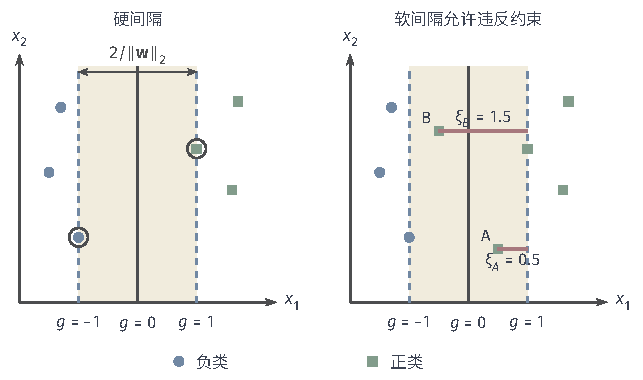
\includegraphics[width=108.850mm]{figures/04-classic-models/00-shared/tikz/classification-svm-margin/figure.pdf}
  \caption{硬间隔与软间隔的教学示意，坐标无量纲。蓝圆为负类，赭方为正类；两个面板都给定$\bm{w}=(1,0)^{\top}$、$b=-2$，黑色实线为决策边界$g=0$，蓝色虚线为间隔边界$g=\pm1$。单侧规范间隔为$1/\lVert\bm{w}\rVert_2=1$，两虚线总宽为$2/\lVert\bm{w}\rVert_2=2$；左图圈出间隔上的样本。右图红色线段直接标出松弛量：A位于$x_1=2.5$，正确分类但在间隔内，$\xi_A=0.5$；B位于$x_1=1.5$，已被错分，$\xi_B=1.5$。右图仅说明给定分界面下的最小松弛量，并非优化后的SVM最优解。}
  \label{fig:classification-svm-margin}
\end{figure}

消去$\bm{\xi}$，式\eqref{eq:classification-svm-soft-primal}等价于
\begin{equation}
  \min_{\bm{w},b}\quad
    \frac12\lVert\bm{w}\rVert_2^2
    +\lambda_{\mathrm{s}}\sum_{i=1}^n
       \max\{0,1-y_i g(\bm{x}_i)\}.
  \label{eq:classification-svm-hinge-objective}
\end{equation}
其中$\ell(z)=\max\{0,1-z\}$是\term{合页损失}（hinge loss）：达到目标间隔以后不再奖励更大的得分，间隔不足时线性增加惩罚。错误一侧的损失继续线性增加而不截断，保持了凸性。它把“最大间隔加违规代价”与“平方范数正则化加经验损失”联系起来。

惩罚参数的数值还依赖损失是求和还是取平均。将式\eqref{eq:classification-svm-hinge-objective}除以$n\lambda_{\mathrm{s}}$，等价目标是平均合页损失加$\lVert\bm{w}\rVert_2^2/(2n\lambda_{\mathrm{s}})$。所以在不同样本量或不同软件约定之间比较超参数时，应先统一归一化方式。较大的$\lambda_{\mathrm{s}}$允许模型付出更大范数来降低训练损失，较小的值更重视范数控制；范数和损失的这种取舍是否适合任务，需要结合数据、表示与验证结果判断。

软间隔的乘子上界来自松弛变量的最优性条件。分别为$1-\xi_i-y_i g(\bm{x}_i)\le0$与$-\xi_i\le0$引入$\alpha_i,\mu_i\ge0$，拉格朗日函数为
\[
  \begin{aligned}
    L={}&\frac12\lVert\bm{w}\rVert_2^2
       +\lambda_{\mathrm{s}}\sum_i\xi_i\\
      &+\sum_i\alpha_i
        \bigl[1-\xi_i-y_i(\bm{w}^{\top}\bm{x}_i+b)\bigr]
       -\sum_i\mu_i\xi_i.
  \end{aligned}
\]
关于$\bm{w},b$的驻点条件仍是式\eqref{eq:classification-svm-stationarity}，关于每个$\xi_i$则要求
\[
  \lambda_{\mathrm{s}}-\alpha_i-\mu_i=0.
\]
结合$\mu_i\ge0$，得到$0\le\alpha_i\le\lambda_{\mathrm{s}}$。取$\bm{w}=\bm{0}$、$b=0$和所有$\xi_i>1$可以严格满足两组不等式，因此不论数据是否可分，Slater条件都成立。消去原始变量后有
\begin{equation}
  \begin{aligned}
    \max_{\bm{\alpha}}\quad&
      \sum_{i=1}^n\alpha_i
       -\frac12\sum_{i,j=1}^n
         \alpha_i\alpha_j y_i y_j
         \bm{x}_i^{\top}\bm{x}_j\\
    \text{s.t.}\quad&
      \sum_{i=1}^n\alpha_i y_i=0,\\
    &0\le\alpha_i\le\lambda_{\mathrm{s}},
      \qquad i=1,\ldots,n.
  \end{aligned}
  \label{eq:classification-svm-soft-dual}
\end{equation}
对偶可行域非空且紧，目标连续，所以对偶最优值可以取得。原始形式同样有最优解；两类非空时，限制目标的水平集可控制$\bm{w}$与$\bm{\xi}$，再由两类约束控制$b$。

软间隔的互补松弛关系多了一组：
\begin{equation}
  \begin{aligned}
    &\alpha_i^{\ast}(m_i^{\ast}-1+\xi_i^{\ast})=0,\\
    &(\lambda_{\mathrm{s}}-\alpha_i^{\ast})\xi_i^{\ast}=0,\\
    &m_i^{\ast}\ge1-\xi_i^{\ast},\qquad \xi_i^{\ast}\ge0.
  \end{aligned}
  \label{eq:classification-svm-soft-kkt}
\end{equation}
联合原始与对偶可行性，可以逐项读出
\begin{equation}
  \begin{aligned}
    \alpha_i^{\ast}=0
      &\ \Longrightarrow\
        \xi_i^{\ast}=0,\quad m_i^{\ast}\ge1,\\
    0<\alpha_i^{\ast}<\lambda_{\mathrm{s}}
      &\ \Longrightarrow\
        \xi_i^{\ast}=0,\quad m_i^{\ast}=1,\\
    \alpha_i^{\ast}=\lambda_{\mathrm{s}}
      &\ \Longrightarrow\
        m_i^{\ast}=1-\xi_i^{\ast}\le1.
  \end{aligned}
  \label{eq:classification-svm-soft-cases}
\end{equation}
边界上的样本可以出现在三种乘子状态中：$\alpha_i^{\ast}=0$允许$m_i^{\ast}=1$，$\alpha_i^{\ast}=\lambda_{\mathrm{s}}$也允许$\xi_i^{\ast}=0$且$m_i^{\ast}=1$。反过来，$m_i^{\ast}>1$必有$\alpha_i^{\ast}=0$，$m_i^{\ast}<1$必有$\alpha_i^{\ast}=\lambda_{\mathrm{s}}$，而$m_i^{\ast}=1$时乘子可以是盒约束中的任意值，只要整体KKT系统成立。达到上界的乘子因此可能对应边界点、间隔内的正确样本或错分样本，需要结合$m_i^{\ast}$才能区分。

范数项依然只对$\bm{w}$严格凸，足以保证最优权重唯一，却不能保证偏置唯一。一个简单反例是两个输入都为零，标签分别为$+1$与$-1$。此时$\bm{w}^{\ast}=\bm{0}$，任意$b\in[-1,1]$都使总合页损失为$2$，因此都最优。该情形也说明，软间隔可能得到常值得分；只有$\bm{w}\ne\bm{0}$时，才可以继续用$1/\lVert\bm{w}\rVert_2$解释规范间隔的几何宽度。

若存在$0<\alpha_k^{\ast}<\lambda_{\mathrm{s}}$的\term{自由支持向量}（free support vector），它既参与决策又未碰到乘子上界，可用$m_k^{\ast}=1$恢复偏置。若没有这种样本，就应使用KKT给出的偏置区间。令$h_i=\sum_j\alpha_j^{\ast}y_j\bm{K}_{j,i}$，则$\alpha_i^{\ast}=0$要求$y_i(h_i+b)\ge1$，$\alpha_i^{\ast}=\lambda_{\mathrm{s}}$要求$y_i(h_i+b)\le1$。正标签的前一条件与负标签的后一条件给出下界，另两种组合给出上界；从两组界的交集中选择一个$b$，才是完整的恢复规则。该区间不一定收缩为单点。

SMO的一元目标与误差公式不变，但可行区间必须同时保证两个乘子都位于盒子内。令$s=y_i y_j$，新的$\alpha_j$区间为
\begin{equation}
  \begin{aligned}
    s=+1:\quad
    L&=\max\{0,\alpha_i^{(t)}+\alpha_j^{(t)}
                    -\lambda_{\mathrm{s}}\},\\
    H&=\min\{\lambda_{\mathrm{s}},
                    \alpha_i^{(t)}+\alpha_j^{(t)}\};\\
    s=-1:\quad
    L&=\max\{0,\alpha_j^{(t)}-\alpha_i^{(t)}\},\\
    H&=\min\{\lambda_{\mathrm{s}},
           \lambda_{\mathrm{s}}+\alpha_j^{(t)}-\alpha_i^{(t)}\}.
  \end{aligned}
  \label{eq:classification-svm-smo-soft-interval}
\end{equation}
这是由盒约束与等式约束共同截出的区间，通常小于$[0,\lambda_{\mathrm{s}}]$。使用式\eqref{eq:classification-svm-smo-update}剪裁并回代即可；当$\eta=0$时，这里的区间总是有限，可以直接比较端点目标。偏置仍按式\eqref{eq:classification-svm-smo-bias}计算，但优先使用更新后满足$0<\alpha_i<\lambda_{\mathrm{s}}$或$0<\alpha_j<\lambda_{\mathrm{s}}$的样本；二者都不自由时，可暂取两个候选偏置的平均，停止时再按全体KKT条件核验。

在可分数据上，足够大的有限惩罚就能使软间隔与硬间隔精确对应。取任意硬间隔最优乘子$\bm{\alpha}^{\mathrm{h}}$，若$\lambda_{\mathrm{s}}>\max_i\alpha_i^{\mathrm{h}}$，则硬间隔原始解连同$\bm{\xi}=\bm{0}$、$\bm{\alpha}^{\mathrm{h}}$和$\mu_i=\lambda_{\mathrm{s}}-\alpha_i^{\mathrm{h}}>0$满足软间隔KKT。由强对偶它也是软间隔最优解，而且正的$\mu_i$迫使所有最优松弛量为零。若数据不可分，则无论把惩罚增大到多少，都不能恢复一个本来就不存在的硬间隔可行解。

\paragraph{$\nu$-SVM：调节间隔与违反比例}
\label{sec:classification-svm-nu-extension}
软间隔惩罚系数衡量一单位间隔违反有多昂贵，却不能直接读成“允许多少训练样本违反间隔”。若希望调节参数与训练中的间隔错误比例、支持向量比例建立联系，可以考虑\term{$\nu$-SVM}（nu-support vector machine）。它把间隔阈值$\rho\geq0$也作为变量，在目标中用参数$\nu$奖励更大的阈值，同时惩罚平均松弛量：
\begin{equation}
  \begin{aligned}
    \min_{\bm{w},b,\rho,\bm{\xi}}\quad&
      \frac12\lVert\bm{w}\rVert_2^2-\nu\rho
      +\frac1n\sum_{i=1}^n\xi_i\\
    \text{满足}\quad&
      y_i(\bm{w}^{\top}\phi(\bm{x}_i)+b)\geq\rho-\xi_i,\\
    &\xi_i\geq0,\qquad \rho\geq0.
  \end{aligned}
  \label{eq:classification-nu-svm}
\end{equation}
消去原始变量后，可学习的仍是训练样本的非负系数，但对偶变为
\[
  \begin{aligned}
    \max_{\bm\alpha}\quad&-\frac12\sum_{i,j}\alpha_i\alpha_jy_iy_jK(\bm x_i,\bm x_j),\\
    \text{满足}\quad&0\leq\alpha_i\leq1/n,\quad
       \sum_i\alpha_i y_i=0,\quad\sum_i\alpha_i\geq\nu.
  \end{aligned}
\]
最后一个不等式来自原始问题中的$\rho\geq0$。固定核后可用凸二次规划求系数，再由原始约束和互补松弛恢复偏置及间隔阈值，预测仍对核展开得分取符号。这个目标与软间隔相似，却不是只把惩罚参数换一个名字。

使用时还需结合类别数量检查参数范围：两类训练样本数为$n_+$、$n_-$时，应限制$0<\nu\leq2\min(n_+,n_-)/n$。以下讨论达到精确最优、且最优间隔阈值$\rho^\ast>0$的非退化情形。记最优得分为$g^\ast$，满足$y_i g^\ast(\bm{x}_i)<\rho^\ast$的训练样本称为间隔违反样本；其中也包括已经分类正确、但尚未达到目标间隔的样本。此时，$\nu$是间隔违反样本比例的上界，也是非零对偶系数所对应支持向量比例的下界\scite{scholkopf2000nu}。

这两个方向可以从KKT条件读出。为间隔约束引入乘子$\alpha_i\geq0$。关于松弛变量的驻点条件给出$\alpha_i\leq1/n$；关于$\rho$的驻点条件与$\rho^\ast>0$的互补松弛关系给出
\[
  0\leq\alpha_i^\ast\leq\frac1n,
  \qquad \sum_{i=1}^{n}\alpha_i^\ast=\nu.
\]
这里仍有偏置的驻点条件$\sum_i\alpha_i^\ast y_i=0$，所以正、负两类的乘子总量相同，均为$\nu/2$。每项乘子至多为$1/n$，正类总量因而不超过$n_+/n$，负类总量不超过$n_-/n$。将这两项上界与$\nu/2$比较，就得到前面要求的$\nu\leq2\min(n_+,n_-)/n$；少数类的样本数量限制了两类能够共同承担的乘子总量。这也说明，上述类别数量条件与后面的比例解释都应结合当前模型及最优阈值条件检查。

令$E_\nu=\{i:y_i g^\ast(\bm{x}_i)<\rho^\ast\}$、$S_\nu=\{i:\alpha_i^\ast>0\}$。间隔违反样本的最优松弛量为正，因而乘子必须达到上界$1/n$；另一方面，要把每项至多$1/n$的非负乘子累加到$\nu$，至少需要$n\nu$个非零项。于是
\begin{equation}
  \frac{|E_\nu|}{n}\leq\nu\leq\frac{|S_\nu|}{n}.
  \label{eq:classification-nu-svm-proportions}
\end{equation}
例如，$n=100$、$\nu=0.2$且上述条件满足时，间隔违反样本至多有20个，支持向量至少有20个；这既不表示恰有20个错分样本，也不是对测试错误率的保证。若最优$\rho=0$，这里依据$\sum_i\alpha_i^\ast=\nu$得到的比例解释不能直接沿用。

固定核后，$\nu$-SVM与软间隔SVM使用同一得分族。它改变间隔的选取方式，不增加非线性特征，也仍需要检查核尺度、类别不平衡和独立验证误差。

\subsubsection{多分类：组合二分类器或联合学习}

\label{sec:classification-svm-multiclass}

二分类模型只需判断得分的正负；当候选类别超过两个时，还需要规定多个类别怎样竞争。一个直观的办法是把多分类问题拆成若干个“二选一”的小问题再把答案汇总；另一个办法是让所有类别在同一个优化目标里直接竞争。硬间隔、软间隔和核方法都能作为构件，但“拆成多个二分类器”与“直接优化多类间隔”会得到不同的训练目标。

现在将标签改为$y_i\in\{1,\ldots,C\}$，其中$C\ge3$，类别索引记为$c$。最直接的推广仍然保留二分类求解器，只改变训练任务的组织方式。\term{一对一}（one-vs-one，OvO）为每对类别$c<c'$训练一个分类器$h_{c,c'}$，仅使用标签为$c$或$c'$的样本，共有$C(C-1)/2$个模型。每个模型在这两个类别之间投一票，预测为
\[
  \hat y(\bm{x})
  =\argmax_{c\in\{1,\ldots,C\}}
     \sum_{c_1<c_2}\mathbb{1}\{h_{c_1,c_2}(\bm{x})=c\}.
\]
其中$c_1,c_2\in\{1,\ldots,C\}$，票数并列时采用预先约定的固定规则，例如选择较小类别编号。不同类别对可能作出不相容的局部判断，投票负责把这些判断汇总成一个输出，并不要求它们对应同一个全局概率模型。

\term{一对其余}（one-vs-rest，OvR）为每个类别$c$构造二分类标签：原标签为$c$时取$+1$，其余取$-1$。训练$C$个实值得分函数$g_c$后，使用
\[
  \hat y(\bm{x})=\argmax_{c\in\{1,\ldots,C\}}g_c(\bm{x}),
\]
并固定平局规则。即使所有得分都为负，或多个类别得分为正，这个最大值规则仍能给出类别。它比较的是独立模型的得分，得分尺度与训练中的类别不平衡可能影响比较，因此通常需要统一预处理、损失约定并评估各类别的错误，若要比较类别后验，还需建立并检验相应的概率映射。

图\ref{fig:classification-svm-multiclass}把四个类别展开成具体训练任务。沿着一列看，一对一中的每个类别只参与三个任务；一对其余中，每个样本都参与四个任务，但只有一个任务把它标为正类。沿着一行看，前者忽略不属于当前类别对的样本，后者把所有其他类别合并为负类。这种训练标签的差异，决定了两个组合器面对的子问题并不相同。

\begin{figure}[htbp]
  \centering
  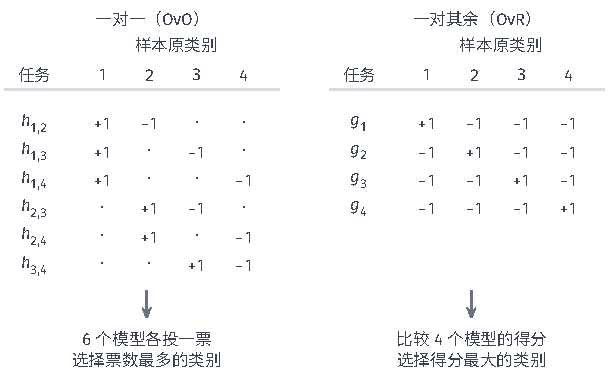
\includegraphics[width=104.027mm]{figures/04-classic-models/00-shared/tikz/classification-svm-multiclass/figure.pdf}
  \caption{四分类任务中的两种二分类组合方式。各行对应一个待训练模型，各列对应样本的原类别；$+1$和$-1$是为该任务重新编码的标签，点号表示该类样本不参与训练。一对一训练6个模型并汇总类别选票，一对其余训练4个模型并比较实值得分。图中给出训练与预测规则，不预设两种方法会产生相同的分类结果。}
  \label{fig:classification-svm-multiclass}
\end{figure}

OvO的模型多、单个训练子问题小，OvR的模型少、每个子问题使用全部样本；总成本因而取决于数据分布和求解器，不能只比较模型个数。

如果希望组合器能够容忍若干二分类判断错误，可以为每个类别安排一个彼此分离的编码。\term{纠错输出码}（error-correcting output codes，ECOC）将类别$c$表示成长度为$q$的码字$\bm{M}_{c,:}$，其中码本$\bm{M}\in\{-1,+1\}^{C\times q}$的各行互不相同，每列同时含两种符号。第$j$列定义一个二分类任务，样本$i$的训练标签为$\bm{M}_{y_i,j}$；训练后得到$q$个二分类器$h_j$。预测时形成输出码$\bm{h}(\bm{x})=(h_1(\bm{x}),\ldots,h_q(\bm{x}))$，再选择最近的类别码字：
\begin{equation}
  \begin{aligned}
    \hat y(\bm{x})
      &=\argmin_c d_{\mathrm{H}}
          \bigl(\bm{h}(\bm{x}),\bm{M}_{c,:}\bigr),\\
    d_{\mathrm{H}}(\bm{u},\bm{v})
      &=\sum_{j=1}^q\mathbb{1}\{u_j\ne v_j\}.
  \end{aligned}
  \label{eq:classification-svm-ecoc}
\end{equation}
这里的\term{汉明距离}（Hamming distance）就是两个码字不一致的位置数。要表示$C$个不同类别，至少需要$q\ge\lceil\log_2 C\rceil$；加入冗余位的目的，是增大不同类别之间的距离，而不只是增加分类器个数。Dietterich与Bakiri系统研究了这种将多分类转换为多个编码位学习问题的方法\scite{dietterich1995ecoc}。

纠错能力可以直接证明。记码本最小类间距离为$\Delta_{\min}$，若真实类别为$c$，输出码与$\bm{M}_{c,:}$相差$e$位，则对任意$c'\ne c$，三角不等式给出
\[
  d_{\mathrm{H}}(\bm{h},\bm{M}_{c',:})
  \ge d_{\mathrm{H}}(\bm{M}_{c,:},\bm{M}_{c',:})-e
  \ge\Delta_{\min}-e.
\]
只要$2e<\Delta_{\min}$，真实码字就比任何其他码字更近。因此至多$\lfloor(\Delta_{\min}-1)/2\rfloor$位错误可以被最近码字解码纠正。这个结论以实际错误位数为条件；若多个二分类器因为相同特征缺陷而同时犯错，冗余编码本身并不能保证错误位数足够小。

另一条路线不再训练彼此独立的二分类器，而是直接优化类别之间的竞争关系。\term{Crammer--Singer多类SVM}（Crammer--Singer multiclass SVM）要求真实类别得分至少比每个错误类别高一个单位间隔，从而在同一目标中学习所有类别权重。

令$\bm{W}=[\bm{w}_1,\ldots,\bm{w}_C]\in\mathbb{R}^{d\times C}$，使用带偏置的版本$g_c(\bm{x})=\bm{w}_c^{\top}\bm{x}+b_c$，相应优化问题为\scite{crammer2001multiclass}。
\begin{equation}
  \begin{aligned}
    \min_{\bm{W},\bm{b},\bm{\xi}}\quad&
      \frac12\sum_{c=1}^C\lVert\bm{w}_c\rVert_2^2
       +\lambda_{\mathrm{s}}\sum_{i=1}^n\xi_i\\
    \text{s.t.}\quad&
      g_{y_i}(\bm{x}_i)-g_c(\bm{x}_i)\ge1-\xi_i,
      \quad c\ne y_i,\\
    &\xi_i\ge0,\qquad i=1,\ldots,n.
  \end{aligned}
  \label{eq:classification-svm-crammer-singer}
\end{equation}
不使用偏置时固定$\bm{b}=\bm{0}$；使用偏置时，可加$\sum_c b_c=0$去掉共同平移的不识别性。消去松弛变量后，每个样本的损失为$\max\{0,\max_{c\ne y_i}[1+g_c(\bm{x}_i)-g_{y_i}(\bm{x}_i)]\}$，即惩罚最强错误竞争者超过允许差距的程度。预测仍取$\argmax_c g_c(\bm{x})$，并可将权重推广到核特征空间。这一凸目标可以用分解法求对偶，线性形式也可用次梯度训练：对每个样本先找得分最高的错误类别；若它违反单位间隔，损失对正确类权重贡献$-\lambda_{\mathrm s}\bm x_i$，对该竞争类贡献$+\lambda_{\mathrm s}\bm x_i$，其余类为零。累计全部样本的贡献，再加上范数项的梯度$\bm w_c$，沿负方向更新各类权重；偏置只累计损失项的相应标量贡献。最强竞争者并列时任选一个仍给出次梯度。这样，训练直接提高正确类相对于错误竞争者的得分，而不独立拟合每个“该类对其余类”的任务。

这一联合目标明确比较了类别之间的相对间隔，OvR则分别比较“该类”与“其余类”。二者的约束数、求解器和数据分解方式不同，训练成本与预测质量也要在相同数据和调参预算下评估。联合建模提供了不同的归纳偏好，并不构成相对于OvO或OvR的普遍性能排序。

这些多分类构造也改变了候选边界。线性OvR与联合多类SVM都按仿射得分的最大值判类，因此每类区域仍是半空间的交。OvO和ECOC先进行若干二分类再解码，各类区域可以由多个分区拼合。这种拼合能够表达单个半空间之外的区域，其能力由可用的二分类划分与解码方式共同决定。训练中的间隔保证若要用于整体分类，还需把错误的二分类比较与最终解码联系起来，不能直接取某个成员的风险作为组合器的风险。



\subsection{模型对比与总结}
\label{sec:classification-geometry-summary}

在同一组输入特征上的二分类问题中，LDA、感知机与线性SVM都用仿射得分形成半空间判断。只看边界的线性形状，无法知道权重来自哪里：LDA从类均值、共享协方差和先验形成得分；感知机在错分点出现时调整当前权重；SVM用范数与间隔损失比较候选边界。相同的得分形式因而不意味着相同的学习目标，也不意味着会从同一训练集选出相同边界。

若类条件高斯与共享协方差近似可信，LDA可以同时利用类内相关性并形成后验概率；样本不足以估计完整协方差时，需要收缩或更受限的协方差表示。感知机省去分布拟合，适合直接使用错误反馈作增量更新，但停止预算、访问顺序和历史参数的返回方式会影响结果。SVM在给定表示中显式权衡间隔与违反程度，代价是求解相应优化问题并选择惩罚强度。表\ref{tab:classification-linear-comparison}汇总这些选择条件。

\begin{table}[htbp]
  \centering
  \small
  \begin{tabularx}{\linewidth}{@{}>{\RaggedRight\arraybackslash}p{18mm}>{\RaggedRight\arraybackslash}X>{\RaggedRight\arraybackslash}X@{}}
    \toprule
    模型 & 边界由什么决定 & 主要条件与代价 \\
    \midrule
    LDA & 类均值、共享协方差与类先验 & 高斯假设支持概率解释；协方差估计需足够样本或正则化。 \\
    感知机 & 错分样本触发的权重更新 & 依赖访问顺序；不可分时需停止规则或变体。 \\
    线性 SVM & 范数与间隔损失的权衡 & 硬间隔要求可分；软间隔需选择惩罚强度。 \\
    核 SVM & 特征空间中的间隔 & 核定义相似性；训练与预测开销受样本数和支持向量数影响。 \\
    \bottomrule
  \end{tabularx}
  \caption{线性与核化分类器的比较。LDA 一行指共享协方差的高斯生成模型；Fisher 投影本身不要求高斯分布。比较时还需固定输入表示与评价口径。}
  \label{tab:classification-linear-comparison}
\end{table}

原坐标中的类别关系不能由仿射得分表达时，重复更新参数或调整惩罚都不能补上这种限制。核Fisher判别、核感知机与核SVM改用特征空间内积，分别保留类统计量比较、错分反馈与间隔选择这三种依据。核与输入尺度决定提供哪些关系，各自的学习目标再决定怎样使用这些关系。预测时是否需要保存全部训练样本、更新样本或支持向量，也随方法而异。

若还需要稀疏的概率核预测，相关向量机改用逐基函数的高斯先验与精度学习，其结构与训练见第\ref{sec:classification-rvm}节；它与SVM共享核展开形式，但不使用同一个间隔目标。
